% ** Cuidado: El indice se actualiza al compilar 2 veces. **

% -- Configuración --
\documentclass[10pt, a4paper]{article}
\usepackage[paper=a4paper, left=1.5cm, right=1.5cm, bottom=1.5cm, top=1.5cm]{geometry}
\usepackage[utf8]{inputenc}
\usepackage[spanish]{babel}
\usepackage{float}
\usepackage{mdframed}
% \usepackage[colorlinks=true, linkcolor=blue]{hyperref}
\usepackage{graphicx}
\usepackage{titling}
\usepackage{verbatim} 
\usepackage{tikz}
\usepackage{dsfont}
\usepackage{amsmath}
\usetikzlibrary{chains,fit,shapes}
\newcommand{\ig}[1]{\includegraphics[width=\textwidth]{#1}}
\newcommand{\RNum}[1]{\uppercase\expandafter{\romannumeral #1\relax}}
\usepackage{parskip}
\usepackage{handy}
\usepackage{listings}

 
% -- Documento --
\begin{document}

\setlength{\parindent}{25pt}

	% -- Carátula --
	
	\thispagestyle{empty}
	\title{%
	\huge{Organización del Computador \RNum{2}}\\
	\vspace{4mm}
	\large{Trabajo Práctico 2}
	}
	\date{\vspace{5mm}$2^{\mathrm{do}}$ cuatrimestre de 2013}

	\author{
		\\
		{\rm Emilio Almansi }\\
		\small{ealmansi@gmail.com}
		\and
		\\
		{\rm Miguel Duarte}\\
		\small{miguelfeliped@gmail.com}
		\and
		\\
		{\rm Federico Suárez}\\
		\small{elgeniofederico@gmail.com}
	} % end author
	\maketitle

	
	\vspace{10mm}
	% -- Resumen --
	\begin{abstract}
		\centering{%
			En este documento se analiza las diferencias en rendimiento encontradas para las implementaciones de algunos 
			filtros de imágenes al utilizar instrucciones SIMD de la arquitectura Intel 64.
		}
	\end{abstract}
	\vspace{10mm}

	% -- Indice --

	\tableofcontents

	\newpage
	% -- Contenido --
	% Se edita cada seccion por separado, no hay que cambiar nada acá.
	\section{Introducción}
		% Explicar en que consitió el trabajo (brevemente).
	% - Explicar levemente los criterios usados para la paralelización
	% - Por qué es buena idea usar este tipo de procesamiento en filtros de imágenes. (todos los pixeles reciben exactamente el mismo procesamiento y así en una sola ráfaga se peude levantar y procesar muchos).
	% - Explicar la hipótesis (debería ser n veces mas rápido porque zarasa).
	% - Se intentó estudiar si vale la pena o no el esfuerzo adicional de desarrollo y debuggeo.


	A lo largo de este documento se realizará un análisis consiso sobre el
procesamiento de datos SIMD mediante las intrucciones SSE de la arquitectura
AMD-64. El mismo se hará mediante la comparación de diversas implementaciones
de 3 filtros (2 de video y uno de imágen).

	El procesamiento SIMD consiste en realizar una misma operación sobre varios
datos de manera simultánea. Es decir que lo que se logra es paralelismo a nivel
de datos. Esta clase procesamiento es ideal para realizar filtros sobre imágenes
, porque ahí justamente lo que uno busca es que cada pixel reciba el mismo proceso.


\begin{figure}[h]
\begin{center}
  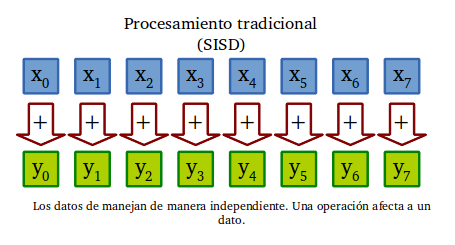
\includegraphics[scale=0.4]{secciones/introduccion/imagenes/SISD.png}
    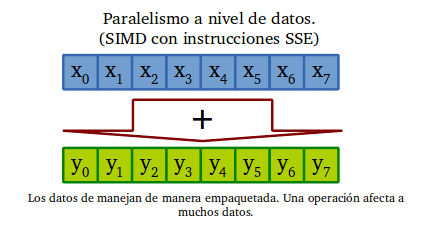
\includegraphics[scale=0.4]{secciones/introduccion/imagenes/SIMD.png}
\end{center}
\caption{Esquemas de procesamiento SISD y SIMD}
\label{fig:SISD-SIMD}
\end{figure}


	Sin embargo para realizar este análisis es imperioso meterse un poco mas adentro.
El comportamiento esperado a priori para estos procesos es una relación inversa entre
el nivel de paralelismo y el tiempo consumido. Es decir, al procesar 4 datos a la vez
uno esperaría obtener que el proceso tarde 4 veces menos tiempo, procesando 8 datos
a la vez 8 veces menos tiempo, etc. Sin embargo esto no siempre ocurre. Durante
este trabajo constantemente se va a intentar explicar que desviaciones se 
produjeron con respecto a este supuesto. Para eso vamos a analizar la arquitectura
intel-64, la velocidad de acceso a memoria, el modo en que se usa la caché,
el medio en el cuál se ejecutan los programas y los algoritmos utilizados entre
otras cosas.

	A lo largo del trabajo se va a ir mostrando como el uso de código de ensamblador
optimizado para el uso de la tecnología SSE produce programas sumamente eficientes. Sin embargo
producir ese código es sumamente trabajoso, mucho mas que usar lenguajes de mas alto nivel como
c o c++. Por ese motivo se intentará hacer otro análisis (tal vez algo menos científico
pero intentando justificar de la manera mas objetiva posible) de cuando vale la pena y cuando no.





	

	\newpage

	\section{Consideraciones generales}
		% comparamos implemtaciones del mismo filtro (versión mas intuitiva posible de c vs asm con SIMD). Esto permite analizar mejor la optimizaciones del compilador. Sobre todo las de icc que tiene introducción automática de SIMD
% En todos los casos se realizó el gráfico C vs ASM (cantidad de clocks y cantidad de líneas de código).
% Como medimos. (menor vs promedio)
% Como se compiló. Compilamos con gcc, con icc, y con diferentes flags.
	% - (aclarar cuales y por qué)
	% - Explicar por qué se puso ICC y no otro(introduce SIMD automáticamente y se supone que es el compilador mas optimo para la arquitectura AMD-64 con procesadores intel).
% cómo se ejcutó. (Mínimas interrupciones, init 2 y kill -9 -1).
% Análisis del código. (object dump).
% - Los tres filtros se programaron pensando en minizar los accesos a memoria incluso en situaciones donde producía cálculo extra.


\subsection*{Método de trabajo}

	A la hora de implementar los filtros se tuvieron algunas consideraciones generales 
para poder explicar los resultados de manera correcta, para manetener la coherencia
interna dentro del trabajo y para tener bases firmes en las que basarnos para sacar
conclusiones.
	Siguiendo esta idea todo lo implementado sigue los siguientes criterios:
		\begin{itemize}
			\item Todas las implementaciones de C intentan ser lo mas intuitivas posibles. No se
			utilizaron optimizaciones demasiado extrañas. Intentan ser una traducción bastante
			fiel de la descripción en lenguaje natural del enunciado a C. Decimos esto para
			poder analizar de manera pura la diferencia entre los dos paradigmas. Además
			a la hora de analizar los archivos objeto creados por los compiladores
			tener un algorítmo simple ayuda a hacer un análisi mas simple y consistente.
			Por otra parte da libertad al compilador para meter tanta paralelización como pueda
			de tal manera que los diferentes compiladores puedan introducir ellos las optimizaciones
			en lugar de respetar un esquema previo.

			\item Todas las implementaciones en asm se escribieron intentando minimizar al máximo
			los accesos a memoria. Una vez dentro del ciclo sólo se accede a memoria para buscar
			datos y para escribir datos. La razón de esto es que los accesos a memoria son lentos,
			por lo que en general cuando se busca performance es buena idea evitarlos. Sin embargo
			en cada implementación se va a analizar si esto fue una decisión acertada o no.
			
			\item Todos los códigos de C se compilaron con 2 compiladores distintos:
				\begin{itemize}
					\item GNU C Compiler (GCC): Se eligió por ser un compilador libre, conocido, popular
					, sumamente versatil y porque es capaz de realizar una gran gama de optimizacizaciones, probablemente
					todas aquellas que se pueden realizar sin acceder al micro código de intel.

					\item Intel C++ Studio XE (ICC): Este compilador introduce de manera predeterminada código
					que aprovecha la tecnología SSE. Es decir que de manera predeterminada genera código objeto
					que realiza paralelismo a nivel de datos. Además realiza optimizaciones de altísima calidad
					aprovechando los detalles del micro-código.

				\end{itemize} 
				
			Además si bien siempre se compiló indicándole al compilador que use instrucciones SSE4.3 además
			se hicieron 2 versiones distintas con cada compilador: Una con optimizaciones agresivas y otra sin
			ellas. Para la primera usó el flag -Ohard, mientras que para la segunda se dejó el comportamiento
			predeterminado.

		\end{itemize}

\subsection*{Método de testeo y medición}

	A la hora de realizar las mediciones de tiempo se intentó armar el ambiente mas
ameno posible. Para esto antes de realizar los tests se mataron todas las aplicaciones
no vitales para el sistema operativo, incluída la interfaz gráfica, acceso a internet y
toda esa clase de cosas (init 1, kill -9 -1). Además se desconectaro todos los periféricos
innecesarios.

	Las mediciones se repitieron entre 50 y 100 veces (según el filtro). Estos números se
decidieron en base a prueba y error. Eliminando los valor atípicos de esa cantidad
de valores hacia arriba la variación de la media era despreciable (menor al 0.5)

	




	\newpage

	\section{Filtro de color}
		\subsection{Descripción del filtro}

El filtro de color es una transformación sobre imágenes a color que tiene el efecto de decolorizar o pasar a escala de grises todos los píxeles de la entrada cuyo color no esté dentro de un rango de colores especificado. En la figura \ref{fig:filtro-color-ejemplo} se observa un ejemplo de funcionamiento típico.

\begin{figure}[h]
\begin{center}
  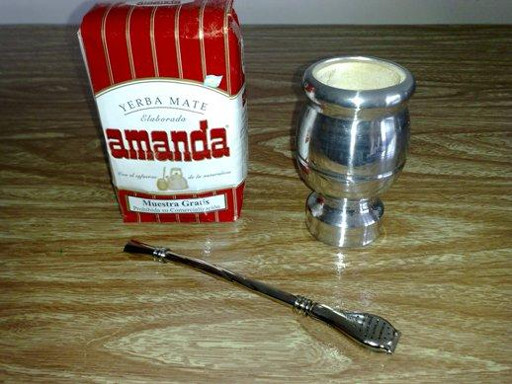
\includegraphics[scale=0.4]{secciones/filtro_color/imagenes/matecocido.jpg}
  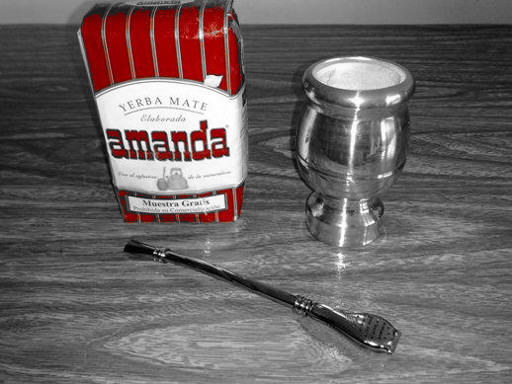
\includegraphics[scale=0.4]{secciones/filtro_color/imagenes/matecocido-fcolor.jpg}
\end{center}
\caption{Imagen antes y después de aplicar el filtro de color con color principal rojo.}
\label{fig:filtro-color-ejemplo}
\end{figure}

La forma en la cual se especifica el rango de colores que deberá permanecer inmutado es mediante la elección de un color principal, cuya codificación RGB se denota con (\param{rc}, \param{gc}, \param{bc}), y un parámetro umbral \param{threshold}. Una vez determinados estos valores, un píxel de la imagen fuente será actualizado por el filtro únicamente si cumple:


\begin{equation} \label{filtro-color-condicion}
\vectornorm{(r, g, b) - (rc, gc, bc)} > threshold 
\end{equation}

donde (\param{r}, \param{g}, \param{b}) es la codificación en RGB del píxel. En particular, de cumplirse esta condición, los tres canales se actualizan de la siguiente forma:

$$ r' = b' = g' = \frac{r + g + b}{3} $$

De esta última expresión se desprende que el color de los píxeles alterados pasa a estar en la escala de grises, ya que los tres canales toman igual valor. Como una observación adicional, queda claro mediante esta especificación que el filtro actúa de forma localizada en sobre cada píxel; su suceptibilidad a ser modificado y su nuevo valor dependen únicamente de su propio valor, y no del de sus vecinos.

\subsection{Implementación en lenguaje C y lenguaje ensamblador}

La implementación en C del filtro se realizó de la forma más sencilla e intuitiva posible; mediante un ciclo que visita una vez a cada píxel de la imagen, de izquierda a derecha y de arriba a abajo, evaluando la condición y modificando su valor de ser necesario. Como única optimización elemental, se modificó la condición (\ref{filtro-color-condicion}) por la siguiente condición equivalente:

$$\vectornorm{(r, g, b) - (rc, gc, bc)}^2 = (r - rc)^2 + (g - gc)^2 + (b - bc)^2 > threshold^2$$

La modificación evita el cálculo de una raíz cuadrada, sin incurrir en el riesgo de exceder el rango del tipo de datos utilizado ya que el máximo \param{threshold} que no hace a la condición trivialmente falsa es $\sqrt{195075} \approx 441$ (el valor máximo que puede tomar la expresión de la izquierda es $255^2 + 255^2 + 255^2 = 195075$), por lo que cualquier valor mayor se puede reducir a $442$.

La implementación en lenguaje ensamblador mantiene esencialmente el mismo procedimiento, con la salvedad de que fue adaptado para procesar cuatro píxeles en simultáneo mediante el uso de operaciones SIMD. Se recorre la matriz en el mismo órden descripto previamente, realizando lecturas de 16 bytes por iteración (equivalente a 5 píxeles y un byte sobrante).

El procesamiento simultáneo se limitó a cuatro píxeles ya que en nuestra implementación se computa la distancia entre un píxel y el color principal explícitamente, cuyo valor cae en el rango $0, ... \,195075$. Este último valor no cabe en un entero de 16 bits, precisándose un \tipo{double word} para almacenar ese resultado temporal; esto implica un total de hasta cuatro valores de distancia en un registro XMM. Por esta razón, además sería similar trabajar con el tipo de datos \tipo{float} ya que también caben hasta cuatro por registro de 128 bits.

De esta forma, el procedimiento realizado en cada iteración consiste en (para cada uno de los cuatro píxeles en simultáneo) comparar el valor de la distancia con el \param{threshold}, y calcular el promedio de los tres canales, actualizando luego sus valores según la siguiente expresión informal:

$$\text{valor\_original} \land \lnot \text{cumple\_condicion} + \text{promedio} \land \text{cumple\_condicion}$$

Esto permite expresar el equivalente a una expresión del tipo \textbf{if}-\textbf{then}-\textbf{else}, en el lenguaje del procesamiento simultáneo. El cómputo de los flags con el resultado de las comparaciones y del promedio se puede describir mediante el pseudo-código de la figura \ref{fig:pseudocodigo-filtro-color}.

\begin{figure}[h]
	\begin{mdframed}
	\begin{center}
		\begin{lstlisting}
		prom := [0,0,0,0] 			// enteros doubleword
		dist := [0,0,0,0]
	
		desempaquetar el rojo de cada pixel a un double word
		rojos := [r4, r3, r2, r1]
	
		prom += rojos
		rojos -= [rc, rc, rc, rc]
		rojos *= rojos
		dist += rojos
	
		repetir para verdes
		repetir para azules
	
		prom := prom / 3
		dist := dist > [threshold, threshold, threshold, threshold]
		empaquetar prom y dist a formato pixeles

		resultado := datos AND NOT dist
		resultado += prom AND dist
		\end{lstlisting}
	\end{center}
	\end{mdframed}
	\caption{Pseudo-código de la implementación en lenguaje ensablador del filtro color.}
	\label{fig:pseudocodigo-filtro-color}
\end{figure}

Para simplificar la implementación, se asumió que la imagen tiene una cantidad de píxeles \emph{múltiplo de 4} ($ancho * altura = 4 * k$); de esta forma, si en cada iteración se procesan 4 píxeles, no es necesario realizar una adaptación en función del tamaño de la imagen. Esta decisión es razonable porque si se admitieran imágenes sin esta característica, habría que procesar solamente 1, 2 o 3 píxeles fuera del ciclo principal, sin alterar significativamente la performance del filtro.

Sin embargo, incluso para una cantidad de píxeles múltiplo de 4, es importante contemplar el \emph{caso borde} que sucede en la última iteración, cuando faltan procesar los últimos cuatro píxeles de la imagen. De realizarse una lectura desde el comienzo del píxel, se leería junto a los píxeles restantes un total de 4 bytes de memoria posteriores al fin de la imagen. Por esta razon, la última iteración se dejó fuera del ciclo principal, realizando un retroceso de 4 bytes en el puntero de lectura, y ejecutando una versión levemente modificada del cuerpo de ciclo de forma tal que procese los píxeles en los últimos 12 bytes del registro, en vez de los primeros.

\subsection{Comparación de performance}
\label{sub:comparaci_n_de_performance_fcolor}

	Se realizaron mediciones en igualdad de condiciones para ambas implementaciones,
según se explicó en la sección de consideraciones generales. En la figura parte de arriba
de la figura \ref{fig:filtro-color-C-vs-ASM} se puede comparar la cantidad de clocks 
consumidos por diferentes implementaciones del mismo filtro.
	La primera barra corresponde a la implementación en asm. Las otras 4 son diferentes
compilaciones de la implementación escrita en C, tal cuál se explicó en la sección de
consideraciones generales.
	
	La parte inferior del gráfico muestra una comparación entre la cantidad de líneas
de código, como para tener una idea de la dificultad en la implementación en cada
lenguaje. Desde ya que esta no es una comparación precisa ni objetiva, sin embargo da una
idea de que la lógica es mucho mas compleja en la versión de ensamblador.




\begin{figure}[H]
\begin{center}
  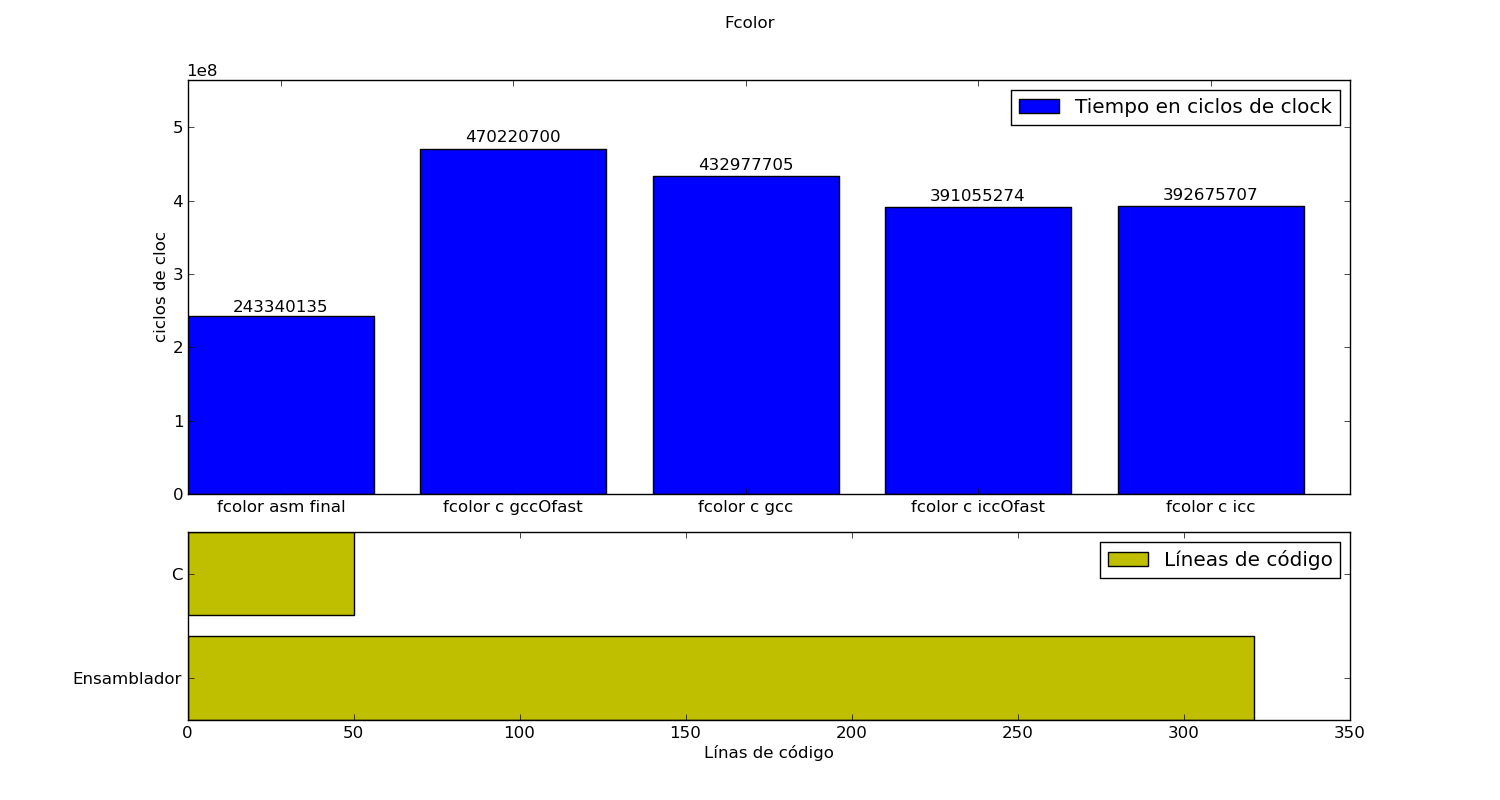
\includegraphics[scale=0.5]{secciones/filtro_color/graficos/fcolor.png}
\end{center}
\caption{Comparación de performance (superior) y cantidad de líneas de código (inferior) entre versión C básica y versión ASM básica.}
\label{fig:filtro-color-C-vs-ASM}
\end{figure}

El resultado muestra un incremento en velocidad de ejecución de aproximadamente 8 veces. Es importante destacar que esta mejora cercana a un orden de magintud no deviene de un cambio algorítmico, sino simplemente de un uso más provechoso de los recursos del procesador; particularmente, las operaciones SIMD. El costo de esta optimización recae en mayor tiempo de desarrollo, lo cual se puede retratar utilizando como indicador la cantidad de líneas de código mediante la figura \ref{fig:filtro-color-C-vs-ASM} (parte inferior).


\subsection{Optimizaciones en código C}
\label{sub:filtro-color-optimizaciones-c}

El siguiente gráfico muestra la diferencia entre compilar este filtro con los distintos niveles de optimización
que ofrece el compilador GCC.\footnote{Ver http://gcc.gnu.org/onlinedocs/gcc/Optimize-Options.html.}:

\begin{itemize}
	\item \textbf{-O/-O1}: Optimizar. Intentar reducir el tamaño de código y tiempo de ejecución sin realizar optimizaciones que requieran mucho tiempo de compilación.
	\item \textbf{-O2}: Optimizar aún más. Se incrementa el tiempo de compilación y la performance del código generado. Esto incluye, por ejemplo, la eliminación del checkeo por punteros inválidos (delete-null-pointer-checks).
	\item \textbf{-O3}: Optimizar incluso más. Incluye, por ejemplo, inlining automático de funciones y vectorización de loops (ftree-loop-vectorize).
\end{itemize}


\begin{figure}[H]
\begin{center}
  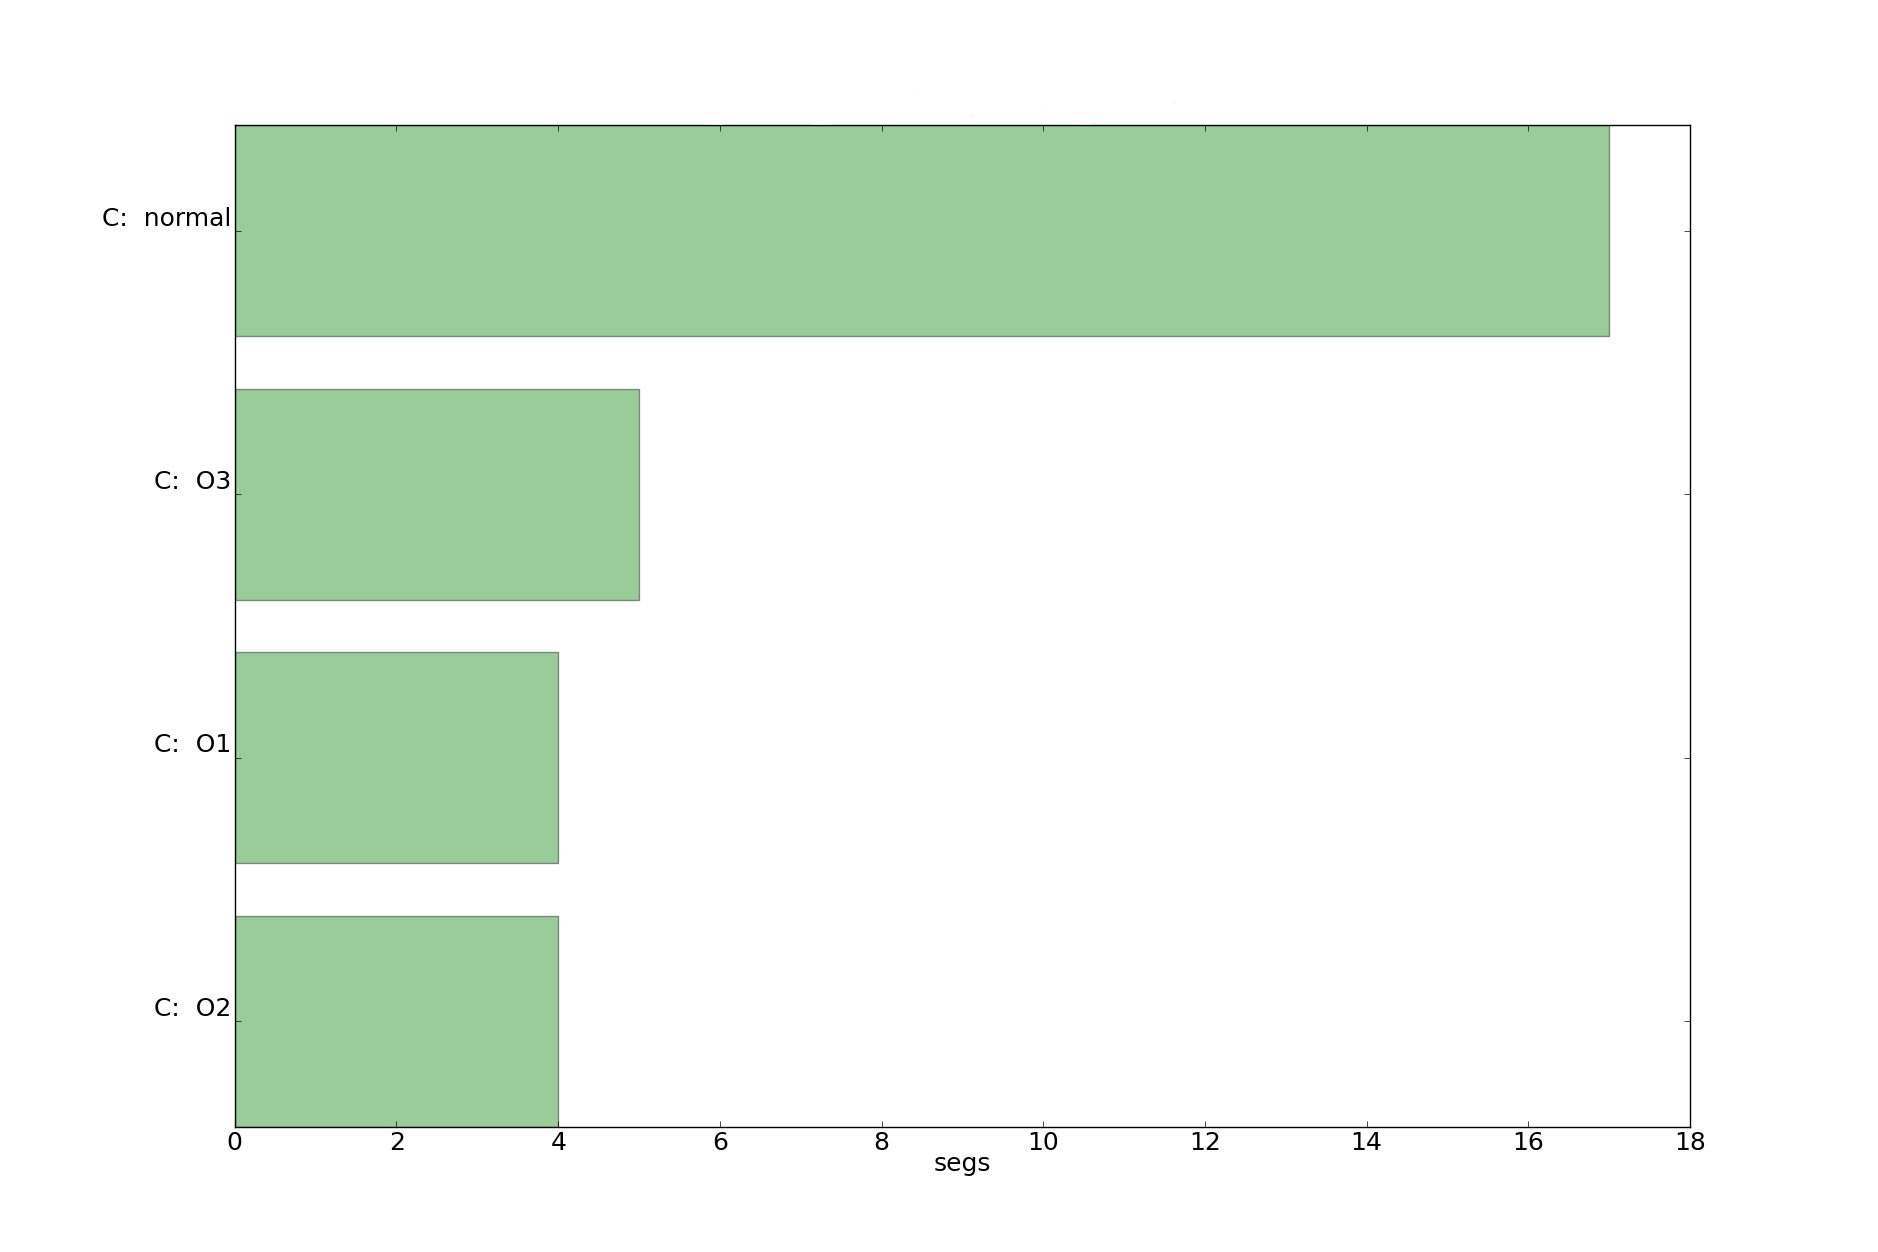
\includegraphics[scale=0.35]{secciones/filtro_color/graficos/C_normal_O1_O2_O3.png}
\end{center}
\caption{Comparación de performance entre la versión C compilada con distintos flags de optimización.}
\label{fig:filtro-color-C-vs-Os}
\end{figure}

El incremento en performance al activar las optimizaciones del compilador es notable, reduciendo a aproximadamente un cuarto el tiempo de ejecución en todos los casos. Sin embargo, la relación de performance entre los resultados con distintos flags no fue la prevista; el flag \textbf{O3} generó código menos performante que las otras optimizaciones\footnote{Muchas fuentes argumentan que el flag O3 no necesariamente genera código más eficiente que O2, e incluso que el segundo es más performante en general a partir de GCC 4.x (http://elinux.org/Compiler\_Optimization)}, y el flag \textbf{O2} fue muy levemente superior a la optimización de primer nivel. Esto permite aducir que los distintos tipos de optimización automática varían su utilidad según el código que se procesa, por lo cual siempre que se busque optimizar no es una buena estrategia optar por el mayor nivel de optimización \emph{sin realizar una comparación sobre el código particular que se desea optimizar.}

Adicionalmente, se analizaron las diferencias entre el código generado con compilación estándar y el código generado con optimización de tipo O1. La diferencia entre los códigos generados evidencia inmediatamente una característica subóptima del código estándar; \emph{todas} las variables locales se alojan en la pila, incluso habiendo disponibilidad de registros. Los registros se utilizan únicamente como variables temporales, y al final de cada extracto de código se guarda el resultado en un espacio de la pila. El código generado con O1, en cambio, ahorra gran cantidad de esos accesos a memoria. Este comportamiento se ejemplifica con el siguiente extracto (figura \ref{fig:codigo-objeto-filtro-color}).


% esto está atado con alambre...
\begin{figure}[h]
	\begin{mdframed}
	\begin{center}
		\begin{lstlisting}
		mov  eax, DWORD PTR[rbp-0x10]	| imul   r15d,r15d
		mov  edx,eax			| imul   r14d,r14d
		imul edx, DWORD PTR[rbp-0x10]	| add    r14d,r15d
		mov  eax, DWORD PTR[rbp-0xc]	| imul   ebx,ebx
		imul eax, DWORD PTR[rbp-0xc]	| add    ebx,r14d
		add  edx,eax			|			
		mov  eax, DWORD PTR[rbp-0x8]	|			
		imul eax, DWORD PTR[rbp-0x8]	|			
		add  eax,edx			|			
		mov  DWORD PTR [rbp-0x4],eax	|			
		\end{lstlisting}
	\end{center}
	\end{mdframed}
	\caption{Código objeto generado con compilación por default (izquierda), y con optimización de tipo O1 (derecha).}
	\label{fig:codigo-objeto-filtro-color}
\end{figure}

Sin embargo, la lógica de flujo del código generado es equivalente. Es decir, las operaciones realizadas y el orden en que se realizan son iguales; se mantiene la forma de recorrer la imagen y el procesamiento píxel por píxel.

	Los otros niveles de optimización cambian esto. Incluso utilizan los registros xmm
pero no de manera óptima.

%Análisis de saltos condicionales

\subsection{Análisis de saltos condicionales}

	Los saltos condicionales son algo absolutamente necesario en la programación.
Si bien existen técnicas para minimizarlos todo diclo $for$ o $while$ consta
básicamente de un salto condicional que se repite una gran cantidad de veces.

	Sin embargo los saltos condicionales que estamos analizando ahora no son
esos sino aquellos que se realizan en medio de la iteración para decidir
si la operación que se va a realizar va a ser una u otra. Es decir que lo
que estamos analizando es como impacta el uso de $if$ en la performance
del filtro.

	
	El primer experimento realizado, entonces, fue sencillamente comentar
el código perteneciente al if. Este análisis en realidad no es justo
ni significativo. Al hacer esto se está comparando un código
que realiza una operación contra otro que no la realiza.
No se obtiene la diferencia entre realizar y no realizar saltos
condicionales sino que se obtiene la diferencia entre realizar
o no realizar una operación completa. Por eso este experimento
se modificó de la siguiente forma:

	A esta altura es importante mencionar que el procesador tiene una enorme
cantidad de optimizaciones para que los saltos condicionales
tengan la máxima performance posible, por eso para realizar este
análisis fue importante tener en cuenta esas optimizaciones y buscar
casos donde le resulte dificil saber que rama del if tiene que tomar.

	Pensando en esto se armaron 2 videos patrón. Ambos consisten
en una imagen repetida en todos los frames del video, lo que
cambia es la imagen.
	En el \textit{patr0n negativo} lo que se hizo fue crear una imagen
que aturdiera lo máximo posible al sistema de predicción de saltos.
La imagen es basicamente una matriz de pixeles que tiene
intercalados blancos con negros de la isguiente manera.

\begin{center}
$
 \begin{pmatrix}
   000000 & FFFFFF & 000000 & FFFFFF & \cdots & 000000 & FFFFFF \\
   FFFFFF & 000000 & FFFFFF & 000000 & \cdots & FFFFFF & 000000 \\
   000000 & FFFFFF & 000000 & FFFFFF & \cdots & 000000 & FFFFFF \\
   FFFFFF & 000000 & FFFFFF & 000000 & \cdots & FFFFFF & 000000 \\
   000000 & FFFFFF & 000000 & FFFFFF & \cdots & 000000 & FFFFFF \\
   \vdots & \vdots & \vdots  & \vdots  & \ddots & \vdots  \\
   FFFFFF & 000000 & FFFFFF & 000000 & \cdots & FFFFFF & 000000 \\
   000000 & FFFFFF & 000000 & FFFFFF & \cdots & 000000 & FFFFFF \\
\end{pmatrix}
$
\end{center}

	La idea con este patrón es que obligatoriamente en una iteración
entra al una rama del if y en la siguiente entra a la otra (si se pasan
los parámetros adecuados).

	El siguiente patrón \textit{patrón positivo} consiste sencillamente en una
imagen blanca repetida durante todo el video. Ambos videos tienen
la misma duración.

	El experimento consiste en comparar cuanto tarda el filtro
en realizarse de manera absoluta (sobre TODA la imagen) sin un
condicional y con un condicional. La idea es comparar peso que 
tiene sólo el salto condicional, pero sólo el salto condicional. Para esto
lo que se hizo fue modificar el código C del filtro añadiendo un 
$else$ al $if$ exactamente igual al $then$. Es decir que la comparación
se realiza pero el resultado es el mismo. La operación siempre se hace.

	Luego se sacó el $if$ pero se dejó la operación. Es decir que acá
también se reliza si o si la operación, sin ninguna clase de condicional
dando vueltas.


\begin{figure}[h]
	\begin{mdframed}
	\begin{center}
		\begin{lstlisting}
		if (Cond) then:    | 
			OPERACION  | 
		else:              | OPERACION
			OPERACION  |
		endif              |
		\end{lstlisting}
	\end{center}
	\end{mdframed}
	\caption{Experimento 1}
	\label{fig:Experimento Saltos}
\end{figure}

	El siguiente gráfico muestra los resultados obtenidos en una ronda de test.
Algunas datos usados para sacar conclusiones no quedan plasmados en este gráfico sin
embargo se explican luego.

\begin{figure}[H]
\begin{center}
  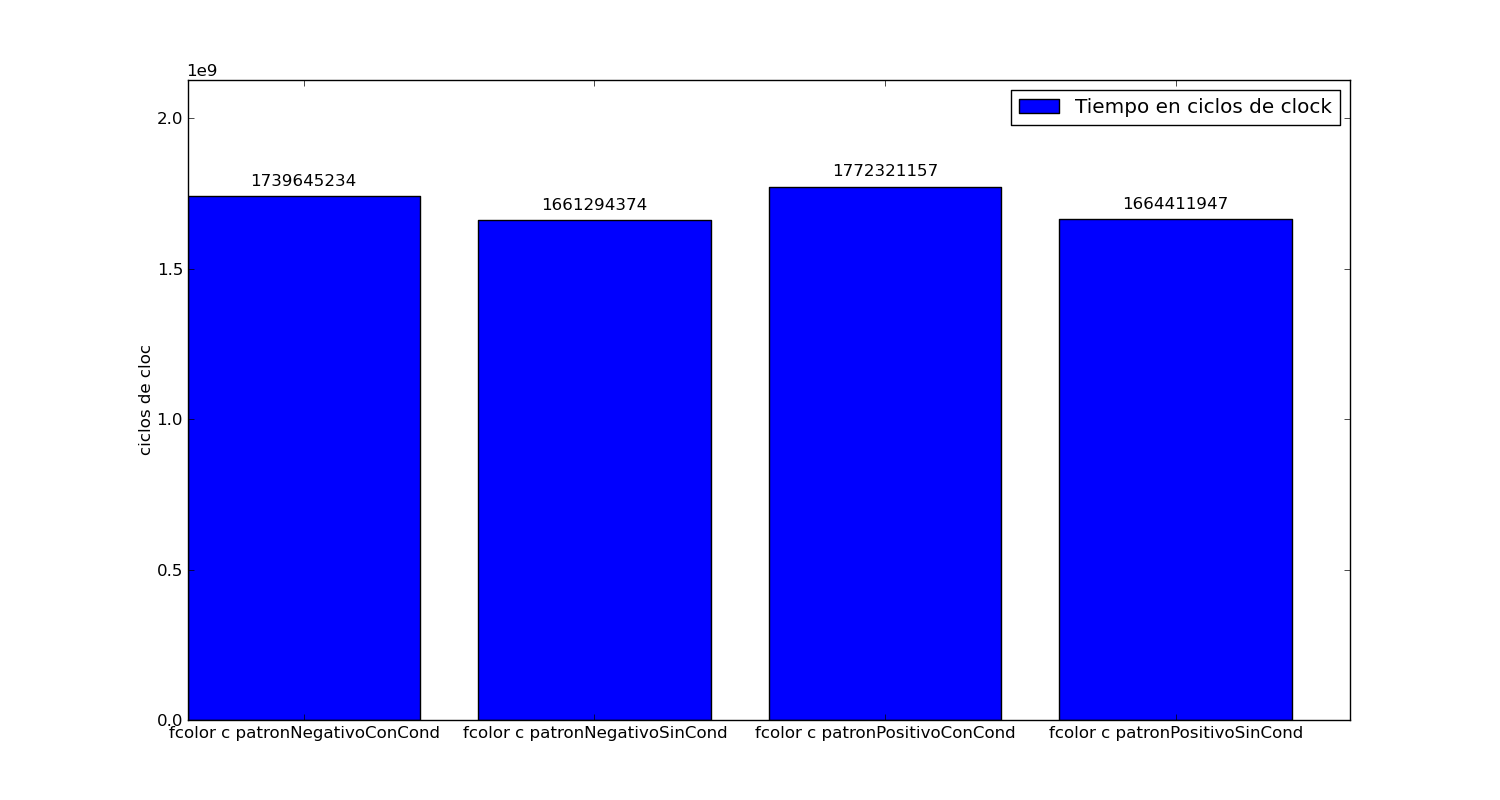
\includegraphics[scale=0.5]{secciones/filtro_color/graficos/performanceExpSaltos.png}
\end{center}
\caption{Resultados de una ronda de test del experimento de saltos}
\label{fig: Tiempos Experimento Saltos}
\end{figure}

	Si bien todas las baterías de test dieron resultados similares el análisis de todos
los resultados logró afirmar aún mas las conclusiones. A continuación
se detallan los comportamientos observados en los test y las concluiones obtenidas:

\begin{itemize}

	\item Como era de esperarse a la implementación sin condicionales no
le afecta la entrada. Es decir, el resultado obtenido para el patrón
positivo y para el patrón negativo fue el mismo. En algunas rondas de
test se realizó mas rápido uno y en otras otro. La diferencia de tiempo
es por cuestiones accidentales a la implementación en si.
	\item Como también era de esperar versión con $if$ resulta levemente
mas lenta. Los reultados oscilaron entre un 4\% y un 6\%. En principio
esto suena extraño, pues sencillamente se están ejecutando 2 o 3 instrucciones
extra para realizar el salto (recordemos que el condicional tiene el mismo código
en las 2 ramas del $if$). Es decir, se podría esperar que la diferencia sea menor.
Sin embargo lo qeu juega acá es el pipeline. Cuando hay condicionales
existen posibilidades de que el pipeline se rompa, además se invierte tiempo
en realizar las predicciones para no romper el pipeline. Esto explica esta diferencia.
	\item Lo mas interesante, tal vez, es la diferencia de tiempo entre
los dos patrones en la implementación con condicionales. Acá ambas ramas
del if son iguales, sin enbargo nos encontramos con una diferencia de performance que oscila
entre un 3\% y un 5\%. Esta diferencia si se vió de manera clara, en todas
las rondas de test el resultado fue el mismo. Eso muestra de manera bastante
que los saltos condicionales adquieren peso en la performance. Otra vez
la explicación de esto es el el pipeline. El patrón positivo es ``Pipeline Amigable'',
mientras que el patrón negitivo no lo es. Es decir el patrón negativo está pensado
para que se desarme el pipeline la mayor cantidad de veces posible.


\end{itemize}


\newpage

\subsection{Optimización en código ASM - Desenrollado de ciclos}
\label{sub:filtro-color-optimizaciones-asm}

Sobre la implementación en lenguaje ensamblador ya descripta, se realizaron dos sucesivas modificaciones para estudiar la técnica conocida como desenrollado de ciclos en su versión más elemental. Esta técnica consiste en minimizar la lógica de flujo, comparaciones y saltos condicionales para ciclos que realizan una gran cantidad de iteraciones. Un ejemplo esquemático se puede ver en la figura \ref{fig:filtro-color-loop-unrolling}.

\begin{figure}[h]
	\begin{mdframed}
	\begin{center}
		\begin{lstlisting}
		for i = 1 .. n		| for i = 1 .. n/k
			F(i)		| 	F(i)
		endfor			| 	F(i + 1)
					| 	...
					| 	F(i + k - 1)
					| endfor
		\end{lstlisting}
	\end{center}
	\end{mdframed}
	\caption{Pseudo-código ejemplo de la técnica loop unrolling.}
	\label{fig:filtro-color-loop-unrolling}
\end{figure}

Siguiendo la notación de la figura, en el caso particular del filtro color, se tomó k = 2, y k = 4, y se realizaron mediciones de performance. Los resultados no fueron provechosos ya que las mejoras observadas fueron menores al 5\%, incluso sin haber considerado el costo adicional de tratar con los casos donde el tamaño de la matriz no es múltiplo de la cantidad de píxeles que se procesan por ciclo, lo cual deterioraría la performance. Este resultado parecería indicar que el costo de la comparación y la escritura al program counter en cada salto no incurren un costo significativo, posiblemente debido a que el procedimiento realiza un único acceso a memoria por iteración (no congestiona la caché) y la posibilidad de ejecución fuera de orden que brinda al procesador (el puntero de lectura que se utiliza para realizar la comparación no se utiliza dentro del cuerpo del ciclo una vez leída la memoria).

	\newpage

	\section{Filtro Miniature}
		\subsection{Descripción del filtro}
\label{sub:miniature_descripcion}

El filtro miniature es un caso particular de la familia de filtros por convolución, en los cuales se procesa una imagen realizando una convolución entre esta y una matriz determinada denominada \emph{kernel}. Las características del \emph{kernel} determinan el efecto resultante sobre la matriz; en este caso, el efecto logrado se conoce como desefoque gaussiano (se puede ver un ejemplo en la figura \ref{fig:filtro-miniature-ejemplo}), y se obtiene mediante el siguiente \emph{kernel}:

\[ \frac{1}{600} *  \left( \begin{array}{ccccc}
  1 &   5 &  18 &   5 &   1 \\
  5 &  32 &  64 &  32 &   5 \\
 18 &  64 & 100 &  64 &  18 \\
  5 &  32 &  64 &  32 &   5 \\
  1 &   5 &  18 &   5 &   1 \end{array} \right)\]

Operativamente, la imagen es procesada mediante una actualización pixel a píxel, reemplazando el valor de cada canal de color del pixel por una combinación lineal del valor de sus vecinos, cada uno ponderado por un coeficiente determinado por un elemento de la matriz. Se toma el elemento central del \emph{kernel} como coeficiente del pixel que se está procesando, y la posición relativa a los demás elementos de la matriz determina a cuál vecino corresponde en la combinación lineal. El factor $\frac{1}{600}$ es una constante de normalización que garantiza que el resultado sea un valor en el rango $[0, 255]$.

\begin{figure}[h]
\begin{center}
  
\includegraphics[scale=0.2]{secciones/filtro_miniature/imagenes/neo.jpg}
  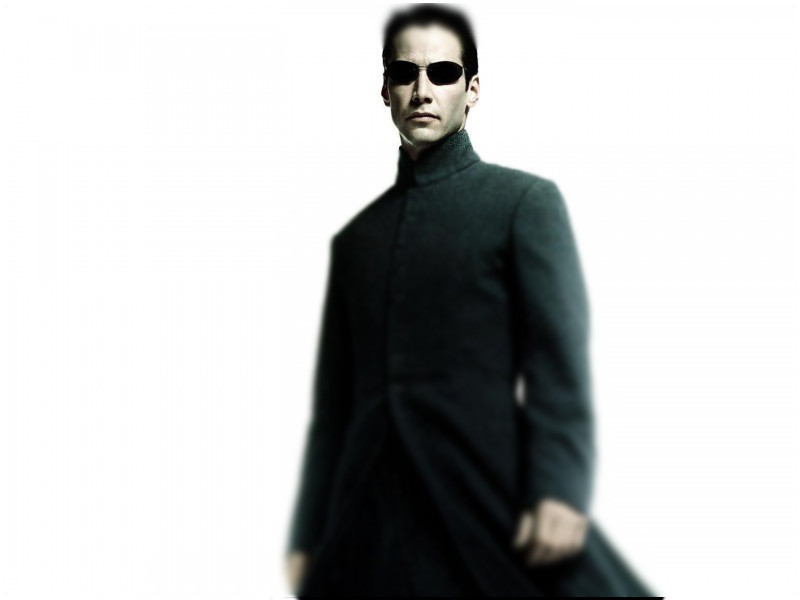
\includegraphics[scale=0.2]{secciones/filtro_miniature/imagenes/neo-miniature.jpg}
\end{center}
\caption{Imagen antes y después de aplicar el filtro miniature con parámetros de banda $0.08$ y $0.25$, y un total de 20 iteraciones.}
\label{fig:filtro-miniature-ejemplo}
\end{figure}

Se incorpora una leve modificación al modelo típico de filtro por convolución, limitando el efecto del filtrado a dos bandas dentro de la imagen; una banda superior, y una banda inferior, dejando la banda central de la imagen inalterada. Se especifican dos parámetros $0 < $ \param{topPlane} $<$ \param{bottomPlane} $ < 1$, de forma tal que las bandas quedan determinadas de esta forma:

\begin{center}
	\raggedright
	\hspace{100pt}\textbf{banda superior:} 	\hspace{10pt}filas 0 ... $topPlane * altura$\\
	\hspace{100pt}\textbf{banda media:} 		\hspace{22pt}filas $topPlane * altura + 1$ ... $bottomPlane * altura - 1$\\
	\hspace{100pt}\textbf{banda baja:} 		\hspace{31pt}filas $bottomPlane * altura$ ... $altura - 1$\\
\end{center}

Adicionalmente, se realizan múltiples iteraciones de filtrado, reduciendo el ancho de cada banda luego de cada iteración por:

\begin{center}
	\raggedright
	\hspace{100pt}$\Delta$\textbf{banda superior:} 	\hspace{10pt}$topPlane * altura / cantIteraciones$\\
	\hspace{100pt}$\Delta$\textbf{banda baja:} 		\hspace{31pt}$(1 - bottomPlane) * altura / cantIteraciones$\\
\end{center}

En el caso de los píxeles del borde, donde no existe el vecindario completo, se optó por exceptuarlos del filtrado, simplificando el procedimiento al saltear las dos primeras y dos últimas filas y columnas.

\subsection{Implementación en lenguaje C y lenguaje ensamblador}
\label{sub:miniature_implementaci_n_en_c}

El filtro se implementó en C mediante un ciclo que visita una vez por iteración a cada pixel de la banda superior y de la banda inferior, y actualizando el valor de sus tres canales de color por la combinación lineal descripta previamente.

Para este filtro, la implementación intuitiva en C resultó particularmente sugerente a la necesidad de buscar formas de optimizar el procedimiento, dado que cada pixel se lee de la memoria hasta 25 veces (una vez por cada vecino) resultando en un tiempo de ejecución prolongado. Además, el tipo de procesamiento realizado por cada pixel es el cómputo de una combinación lineal, para lo cual los procesadores utilizados están altamente optimizados. Realizar esta operación mediante un ciclo es un claro desperdicio de los beneficios brindados por el hardware.

\begin{figure}[h]
\begin{center}
  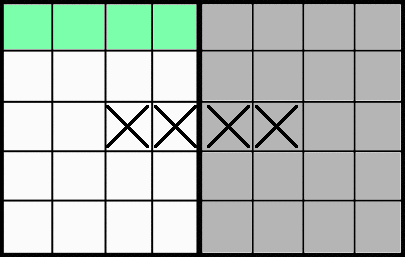
\includegraphics[scale=0.4]{secciones/filtro_miniature/imagenes/grid.png}
  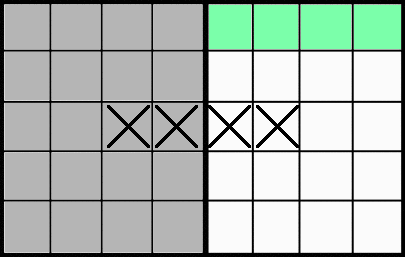
\includegraphics[scale=0.4]{secciones/filtro_miniature/imagenes/grid-inv.png}
\end{center}
\caption{Esquema de procesamiento filas izquierdas, filas derechas.}
\label{fig:filtro-miniature-grillas}
\end{figure}

Para implementar el mismo algoritmo en términos de procesamiento simultáneo, se trabajó con 4 píxeles por cada iteración del ciclo de convolución. Se procuró minimizar los accesos a memoria, mediante el esquema caracterizado por la figura (\ref{fig:filtro-miniature-grillas}): al procesarse los píxeles marcados con cruces, se leen previo al comienzo de la iteración los 20 píxeles sin sombrear. Se inicializan tres acumuladores, uno por cada canal de color, conteniendo la suma parcial \emph{sin normalizar} de los 4 pixeles en simultáneo. Esto es posible ya que el valor de la convolución para un determinado punto jamás excede el valor $255 * 600 = 153000$, el cual cabe en un entero \tipo{doubleword} y por lo tanto se pueden almacenar hasta 4 por registro XMM.

En los acumuladores se suma el aporte de cada uno de los 20 píxeles sin sombrear sobre cada uno de los 4 píxeles marcados con cruces, procesando fila por fila. Es decir, se toma la primer fila (de color verde en el diagrama), se calcula el aporte de cada uno de ellos sobre cada uno de los 4 píxeles con cruz, y se suma al acumulador. La operación se repite para cada uno de los tres canales, y para cada una de las 5 filas sin sombrear.

Para realizar este cálculo, se desempaquetan los tres canales de los píxeles en verde de forma tal de obtener máscaras del tipo:
$$[b_3, b_2, b_1, b_0, b_3, b_2, b_1, b_0]$$
$$[g_3, g_2, g_1, g_0, g_3, g_2, g_1, g_0]$$
$$[r_3, r_2, r_1, r_0, r_3, r_2, r_1, r_0]$$

y luego se realiza el producto interno con máscaras conteniendo elementos de la matriz con la siguiente forma:

$$[c_{30}, c_{20}, c_{10}, c_{00}, c_{31}, c_{21}, c_{11}, c_{01}]$$
$$[c_{32}, c_{22}, c_{12}, c_{02}, c_{33}, c_{23}, c_{13}, c_{03}]$$

donde $c_{ij}$ es el coeficiente del i-ésimo pixel verde sobre el j-ésimo pixel marcado con cruz.

El procesamiento simultáneo en esta etapa se limita a dos píxeles marcados con cruces por vez, ya que un producto del tipo $b_i * c_{ij}$ precisa de hasta un entero de tamaño \tipo{word}, permitiendo calcular hasta 8 productos por vez (y se requieren 4 productos por cada pixel marcado con cruz). Posteriormente, mediante sumas horizontales se obtienen 4 \tipo{doublewords} en un registro XMM, cada uno con una suma del tipo $b_3 * c_3 + b_2 * c_2 + b_1 * c_1 + b_0 * c_0$; este resultado luego se suma al acumulador (de azules, este caso). La operación se repite para cada canal, y para cada fila, obteniendo finalmente el aporte de los 20 píxeles sin sombrear, sobre los 4 píxeles marcados con cruces.

Como aclaración adicional, las máscaras con coeficientes utilizadas para realizar el producto se almacenan en forma de \tipo{bytes}, permitiendo reducir cuatro veces el tamaño requerido de haberse usado \tipo{floats}, y minimizando el costo de lectura.

El próximo paso consiste en leer de memoria los píxeles sobreados. Es importante notar que una vez leídas las filas de la derecha, ya se cuenta con todos los píxeles necesarios para terminar la acumulación sobre los 4 píxeles marcados con cruces; pero adicionalmente, \emph{las 4 filas de la derecha son reutilizadas para la acumulación de lado izquierdo en la próxima iteración}. Esto reduce significativamente la cantidad de lecturas a memoria en comparación a la implementación en C, y además mejora el uso de la memoria caché, ya que al leer los píxeles de lado izquierdo es muy probable que se acelere el acceso al bloque de píxeles del lado derecho.

Para finalizar la actualización, se realiza un proceso similar sobre las filas derechas, aunque es necesario espejar las máscaras de coeficientes utilizadas del lado izquierdo. La suma total luego se normaliza, y se empaqueta en el formato RGB para escribirse en la imagen destino.

La única salvedad o \emph{caso borde} resulta para los últimos 4 píxeles de cada fila, donde se escriben los píxeles del marco que se desea dejar inalterado. Sin embargo, la memoria pisada es válida (pertenece a la imagen), y es sencillo restaurarla realizando una copia desde la fuente; es decir, no hay que realizar retroceso en el puntero o lógica de borde.

\subsection{Comparación de performance}
\label{sub:comparaci_n_de_performance}

Se tomaron mediciones sobre ambas implementaciones con el criterio discutido en la sección de consideraciones generales, y se realizaron gráficos comparando la performance de la implementación en C y la implementación en lenguaje ensamblador.

\begin{figure}[H]
\begin{center}
  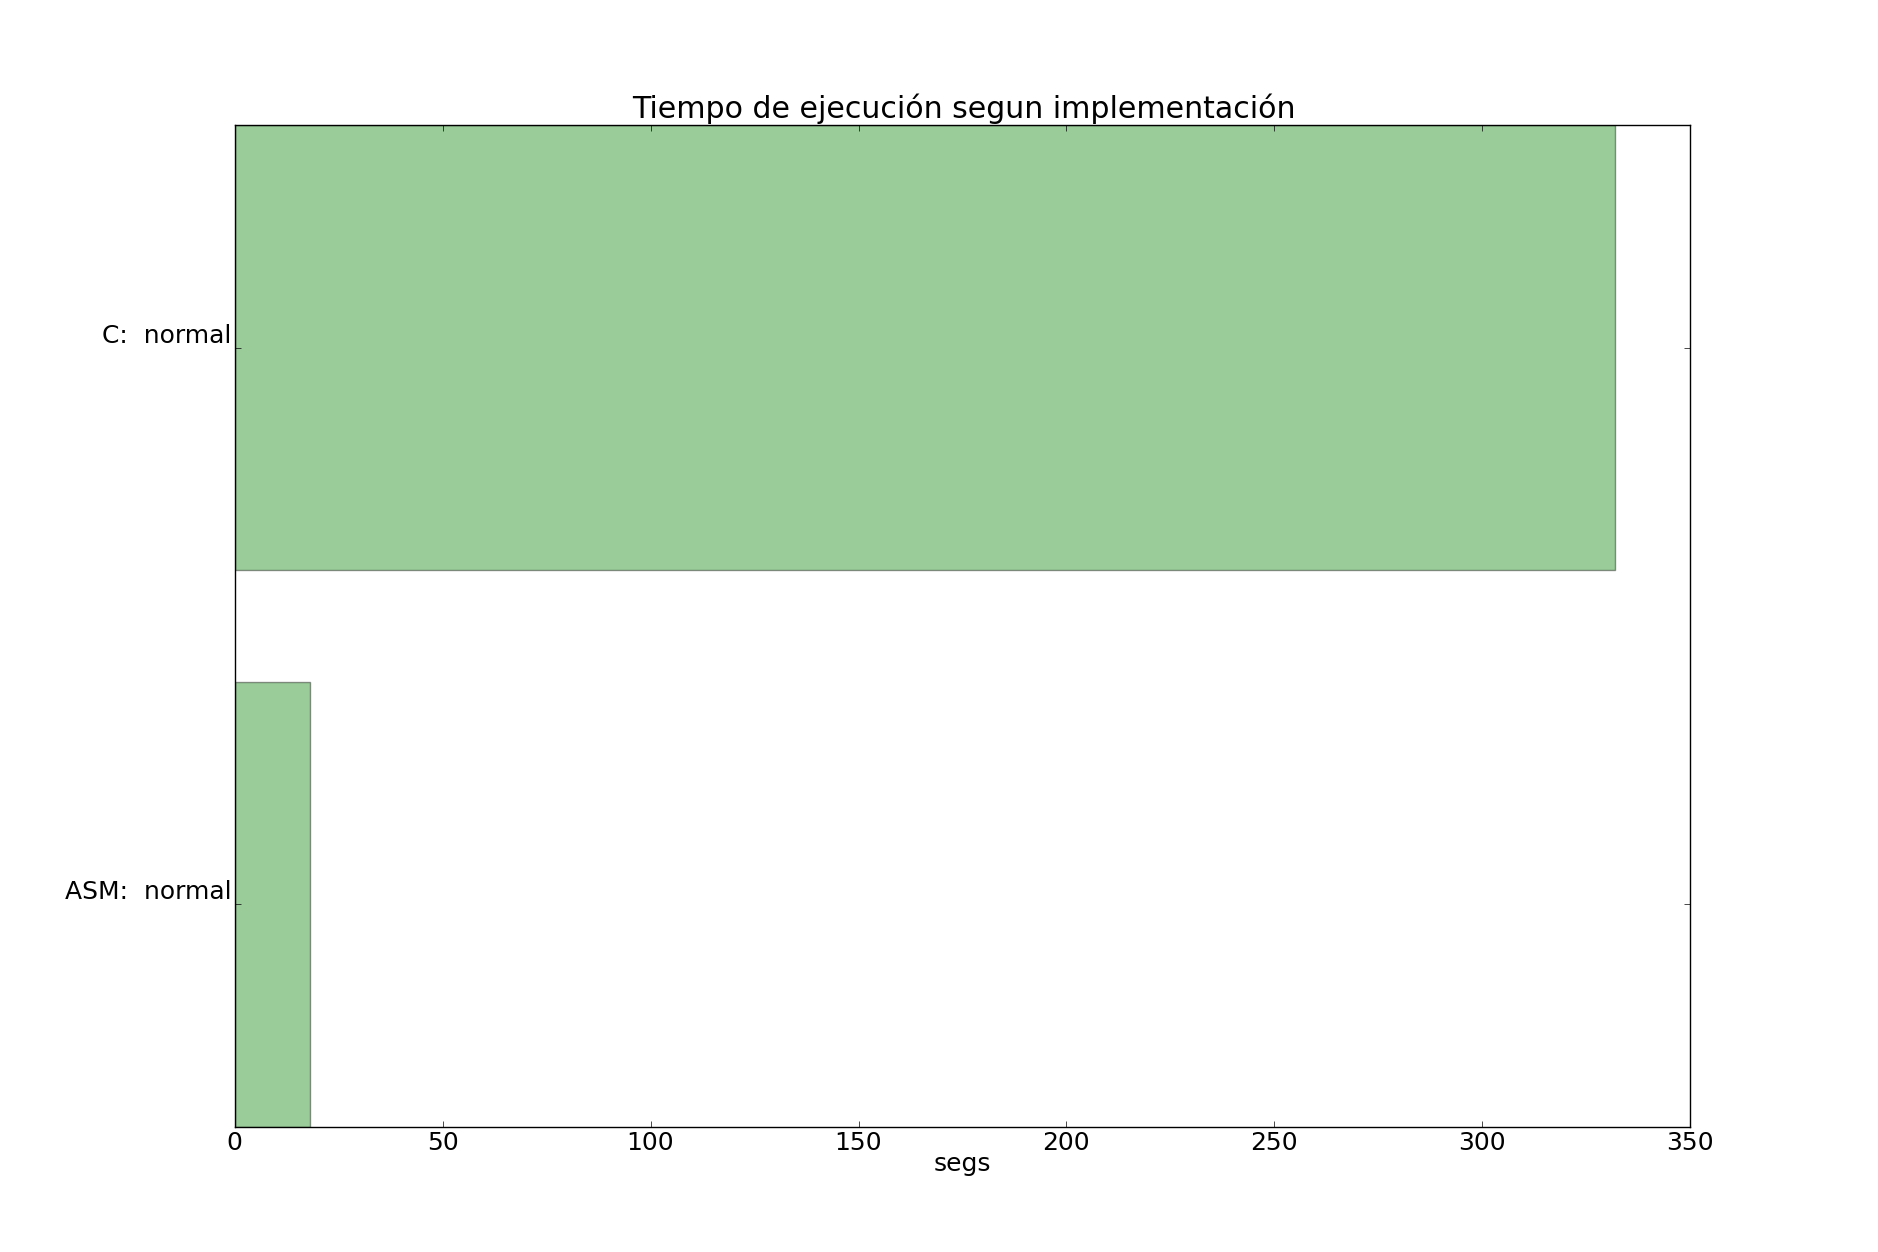
\includegraphics[scale=0.35]{secciones/filtro_miniature/graficos/C_ASM_perf.png}
  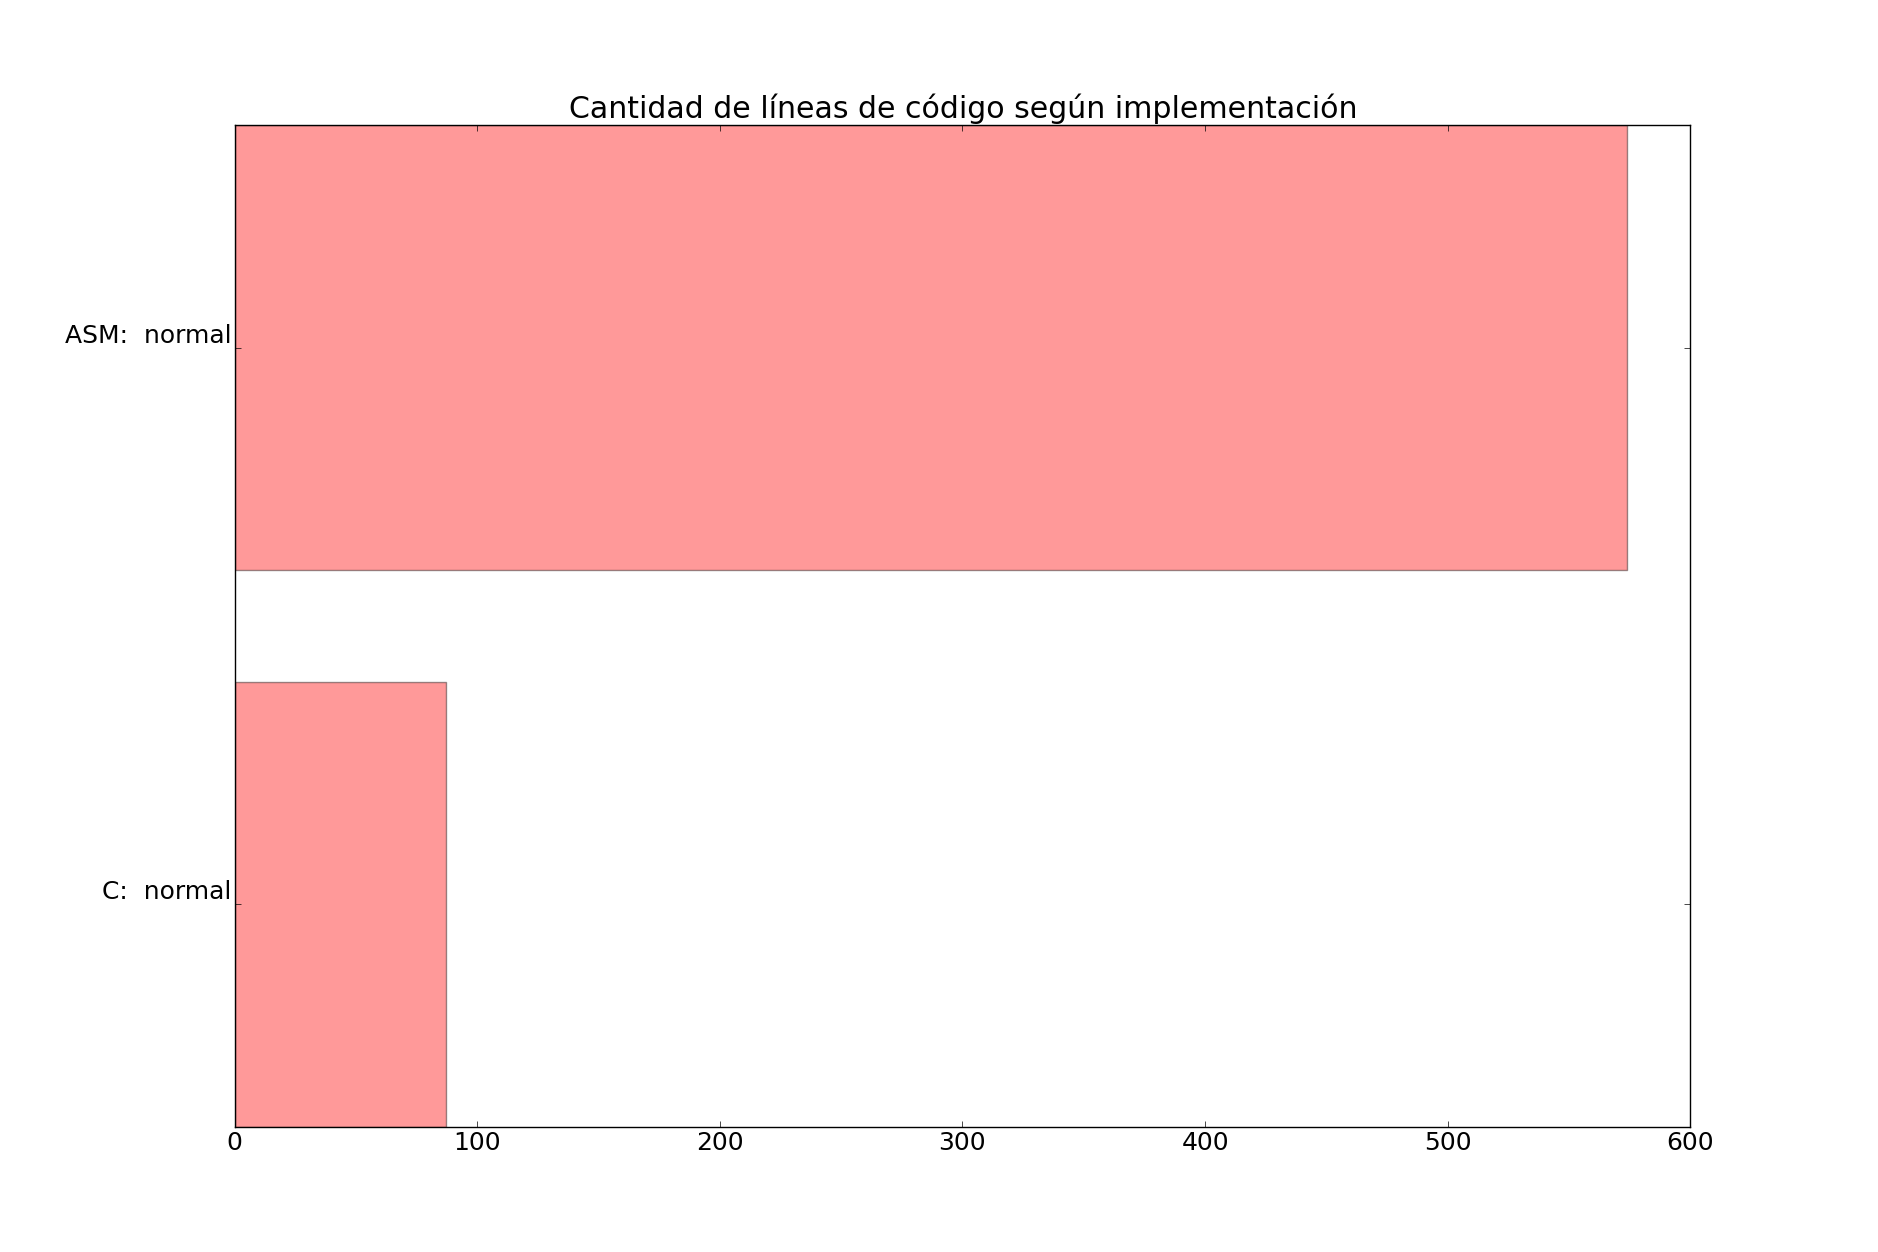
\includegraphics[scale=0.35]{secciones/filtro_miniature/graficos/C_ASM_loc.png}
\end{center}
\caption{Comparación de performance (superior) y cantidad de líneas de código (inferior) entre versión C básica y versión ASM básica.}
\label{fig:filtro-miniature-C-vs-ASM}
\end{figure}

En el caso del filtro miniature, la diferencia de performance entre la versión C y la versión ASM es incluso más radical que para el filtro de color, con mejoras de entre \textbf{x18} y \textbf{x20} veces. La proporción en cantidad de líneas de código, sin embargo, es similar (alrededor de 6 veces). Esto revela que el código C en su versión más intuitiva es particularmente subóptimo para este tipo de procesamiento, dictando que el procesamiento simultáneo y la utilización de los recursos del hardware son fundamentales para cualquier implementación performante de un filtro de convolución.

\subsection{Profiling para la implementación en ASM}
\label{sub:profiling_para_la_implementaci_n_en_asm}

Para estudiar cuáles son los puntos de la implementación en lenguaje ensamblador que es necesario optimizar para mejorar la performance, se realizaron dos mediciones adicionales sobre el código, incluyendo dos variantes:

\begin{itemize}
	\item Todos los movimientos de lectura/escritura a memoria removidos
	\item La lógica de flujo intácta, pero sin realizar la acumulación por filas descripta previamente durante el ciclo de procesamiento.
\end{itemize}

No fue posible medir dentro de la misma ejecución las diferentes partes del código, ya que cualquier mecanismo de medición incluye una costo en clocks que se vuelve significativo si se introduce dentro del ciclo principal. Por lo tanto, se midió el tiempo total de 3 ejecuciones con el código en sus tres variantes. Se incluye en la figura \ref{fig:filtro-miniature-ASM-profiling} un gráfico de circular que \textbf{no} debe interpretarse como el porcentaje de tiempo insumido por cada una de las partes medidas (procesamiento vs lectura/escritura), ya que fueron medidas por separado y sin dudas influyen una en la otra (debido a la ejecución fuera de orden que realiza el procesador). Sin embargo, sí se puede interpretar como el porcentaje de tiempo insumido por cada versión en el total de las 3 ejecuciones, permitiendo estimar una relación entre el costo de las distintas partes.

\begin{figure}[H]
\begin{center}
  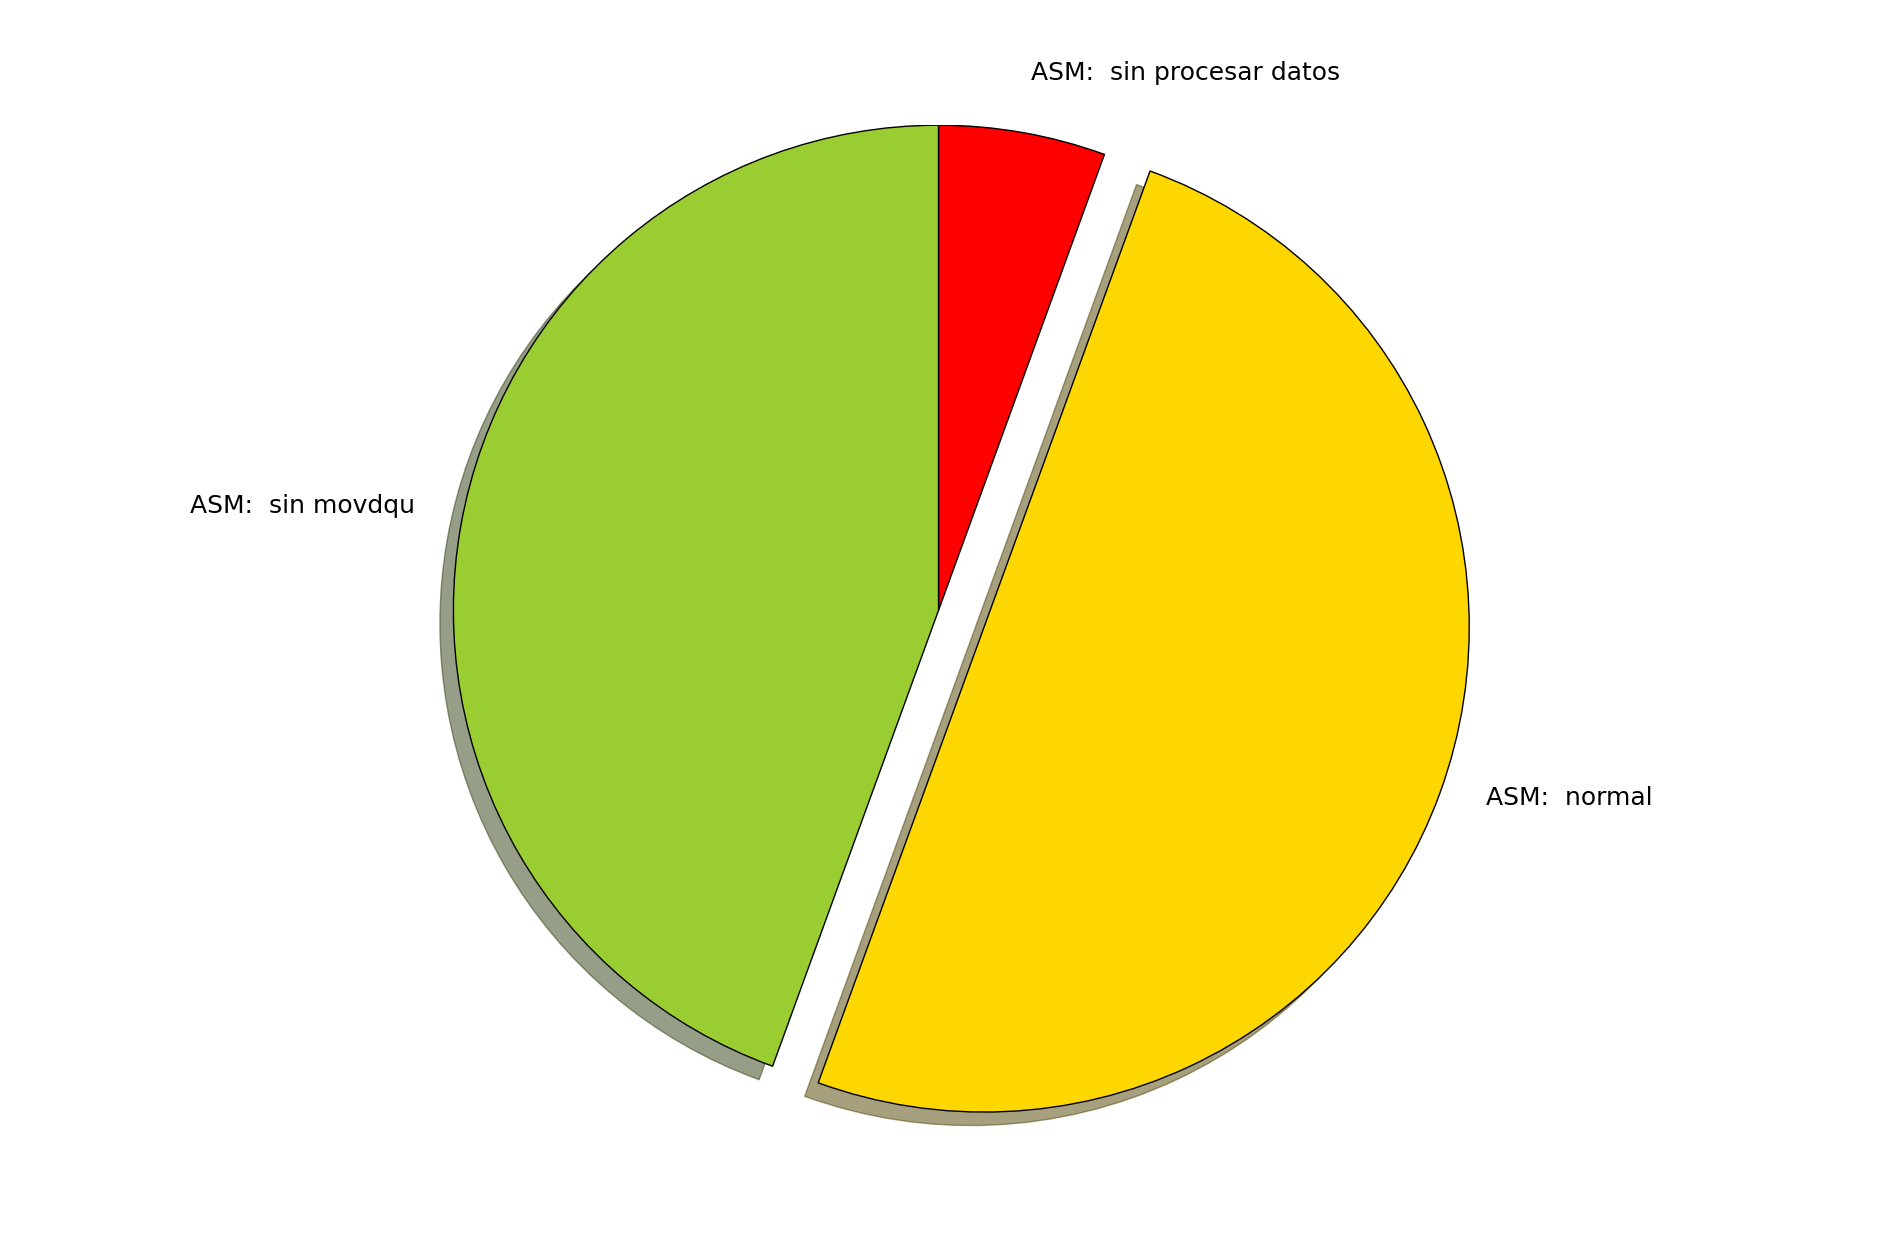
\includegraphics[scale=0.35]{secciones/filtro_miniature/graficos/ASM_normal_sinmovdqu_sinprocesardatos.png}
\end{center}
\caption{Gráfico circular mostrando el porcentaje de tiempo insumido por tres versiones del código ASM: completo, sin lectura/escritura, sin procesamiento.}
\label{fig:filtro-miniature-ASM-profiling}
\end{figure}

Se puede observar en el gráfico que la instancia del programa sin realizar el procesamiento de los píxeles leídos fue signficativamente más veloz que las demás; es decir, la mayor parte del costo total deviene de la etapa de procesamiento. Esta información fue inesperada, ya que la implementación se hizo con una fuerte consideración en evitar las lecturas a memoria, posiblemente incurriendo en costo de procesamiento adicional para evitarlas. Esto indica que un próximo paso en la optimización sería reducir el costo de procesamiento mediante la relajación de la restricción en las lecturas a memoria (posiblemente haciendo uso de mayor número de máscaras, lo cual se evitó por la falta de registros XMM disponibles).
	\newpage

	\section{Decodificación esteganográfica}
		\begin{comment}
	- Comparación c y asm.
		- La mayor diferencia es que se levanta de a más.
	- El tiempo en asm es súper constante porque sólo depende de size. En c mas o menos, explicar por qué.
	- Hay un caso límite. Explicar. Aunque se trata como un chorizo.
	- Explicar optimización del acceso a memoria.
	- Explicar por qué no se puede hacer tanta ejcución fuera de orden. Hay dependencia de datos.
	- ¿Que pesa más?¿Procesamiento o acceso a memoria?

\end{comment}

\subsection{Descripción del filtro}

	El filtro consite en extraer un mensaje codificado detro de la imagen conociendo
, por supuesto la menera en que este está codificado.

	La codificación consiste en cambiar cambiar en cada byte de la imagen los
dos bits menos significativos por los bits del mensaje. Es decir que cada
byte del mensaje de codifica en 4 bytes de la imagen (2 bits en cada imagen).

	Es decir que la imagen está alterada, pero está los cambios son tan leves
que no son visibles al ojo humano. Es mucho mayor la variación de colores que
se produce por ver la imagen en diferentes monitores que la que se produce
por cambiar estos bits.

	Los pares de bits, además tienen una breve codificación individual. Que
se determina mirando los bits 2 y 3 de cada Byte. Es decir que uno sabe
como interpretar los dos bits menos significativos mirando los siguientes
2 bits.

\subsection{Optimizaciones en ASM}

	Este filtro se optimizó mediante la técnica de entubado de código (\textit{software pipelining})
la cual consiste separar un bucle en varios procesos y realizar cada proceso con otros datos.
Lo que se logra con eso es eliminar la dependencia de datos, de manera tal que se favorece
la fácil ejecución. En este punto hay que resaltar que la arquitectura intel-64 tiene un
gran soporte para entubado de código. El procesador realiza todas las operaciones que puede
siempre y cuando estas no tengan dependencia de datos entre si.
	Es importante notar, sin embargo, que el efecto significativo de esto se ve
cuando en el ciclo hay un punto crítico que tarda mucho mas que el resto
del proceso. La idea es aprovechar ese tiempo extra para realizar otras
instrucciones.

	Por ejemplo, en el siguiente caso:

\lstset{language=C}

\begin{lstlisting}[frame=single]  % Start your code-block

for(i=0;i<mucho;i++){

	A(i); //3 ciclos de clock
	B(i); //12 ciclos de clock
	C(i); //2 ciclos de clock
	D(i); //4 ciclos de clock

}
\end{lstlisting}

	Estas operaciones tienen dependencia de datos. Es decir, B(i) no se puede empezar hasta
que A(i) no se haya terminado. Se deben realizar en orden.

	Acá gran parte del tiempo se va en realizar B(i). Hasta que no termine no se puede comenzar
con C(i). Sin embargo si el procesador tuviera otra cosa para hacer que no dependiera de los mismos
datos la realizaría al mismo tiempo que realiza B(i).

	La idea entonces es tener calculado de antemano, antes de entrar a cada iteración, lo necesario
para poder realizar todas las operaciones a la vez en cada iteración. Para esto lo que se hace 
es que cada operación trabaje sobre un dato diferente.

\begin{lstlisting}[frame=single]

fir(i=4; i< mucho; i++){

	A(i);
	B(i-1);
	C(i-2);
	D(i-3);

}

\end{lstlisting}

	Sin embargo para que esto sea posible antes de entrar al ciclo hay que tener ya
calculadas algunas cosas. Por si esto fuera poco el ciclo no termina con todos los datos.
(no llega hasta al \textit{mucho} sino sólo hasta $mucho-4$. Para modificar
esto hay que agregar un prefijo y un sufijo de código. De esta manera quedaría algo
así:

\newpage

\begin{lstlisting}[frame=single]

A(0);A(1);A(2);A(3)
B(0);B(1);B(2);
C(0);B(1)
D(0)

fir(i=4; i< mucho; i++){

	A(i);
	B(i-1);
	C(i-2);
	D(i-3);

}

A(mucho);
B(mucho);B(mucho-1)
C(mucho);C(mucho-1);C(mucho-2)
D(mucho);D(mucho-1);D(mucho-2);D(mucho-3)


\end{lstlisting}

	Como se puede observar hace falta una enorme cantidad de lógica para
lograr un correcto entubado de código. El aumento de rendimiento, sin embargo
es muy significativo pues explota al máximo la capacidad de ejecutar instrucciones
de manera simultanea del procesador.
	

	En el filtro se intentó utilizar el entubado de código de varias maneras.
En un principio se dividió el proceso en 5 etapas: Acceso a memoria por un lado
y por otro los 3 entradas del switch, y una para el acomodado de datos. 
Sin embargo esto no produjo mejoras en la performance, por el contrario disminuyó.
Aplicar la técnica de esta menra conlleva una lógica muy compleja y requiere una gran cantidad
de registros. De esta manera ya no resultaba posible guardar las máscaras en registros estáticos,
por el contrario había que o bien guardarlas en memoria o bien generarlas de manera dinámica
adentro del ciclo.

	Luego se subdividió sólo en 4 etapas, pero otra vez la lógica era realmente compleja
además de que todavía algunas máscaras se tenían que generar de manera dinámica. El aumento de performance
era realmente pobre.

	Luego de estos fracasos se bajó un poco el nivel de ambición y se realizaron sólo 2 etapas. Por un lado 
el acceso a memoria y por el otro todo el resto de los procesos. En realidad esta implementación
tiene mucha lógica, pues los accesos a memoria son lo único que realmente resulta un cuello de botella
en este filtro, todas las otras etapas (salvo tal vez el reacomodado final de datos) son operaciones
sencillas que le consumen pocos ciclos de clock al procesador.



\begin{figure}[h]
\begin{center}
  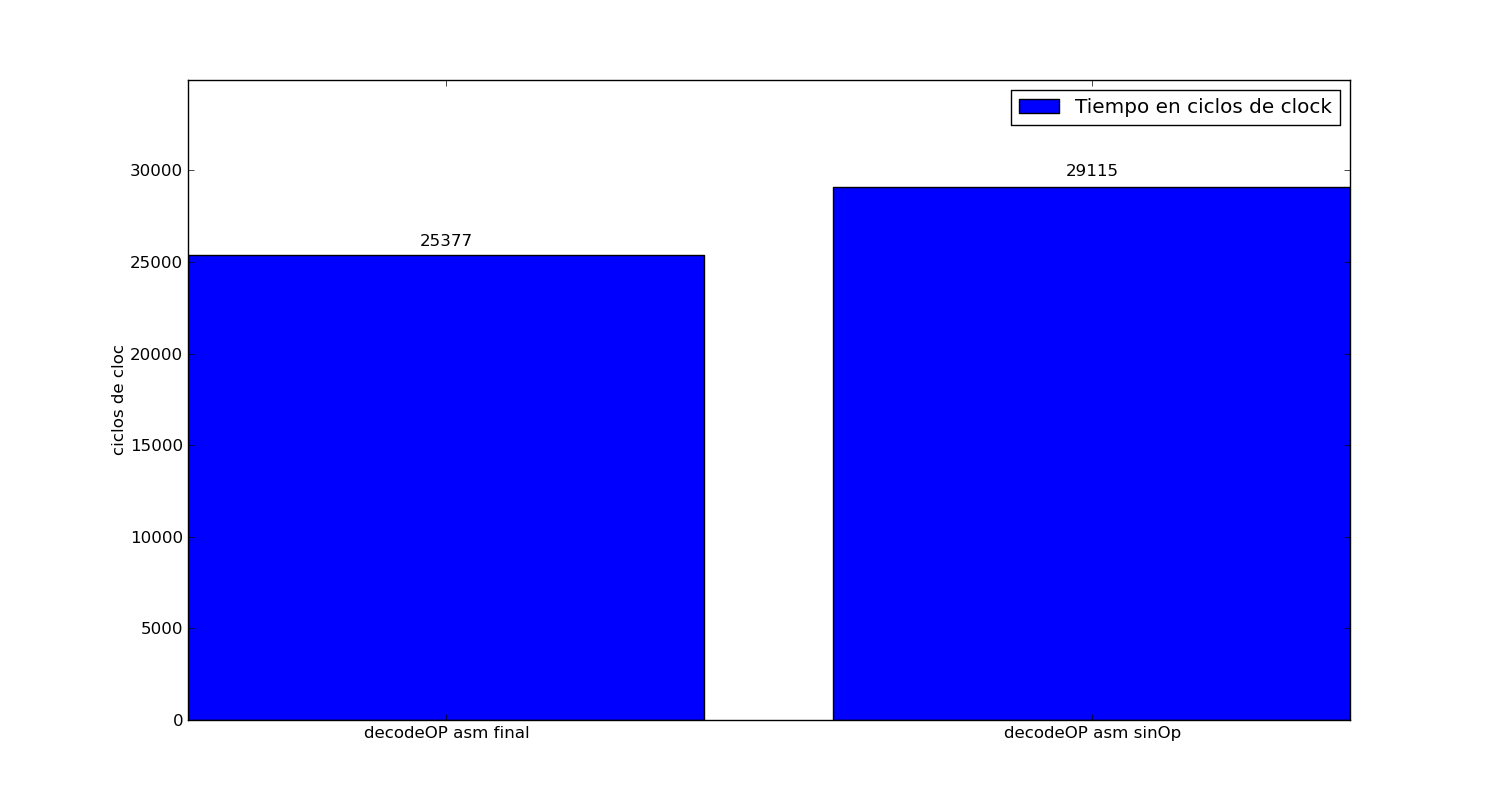
\includegraphics[scale=0.4]{secciones/decodificacion/imagenes/decodeOP.png}
\end{center}
\caption{Diferencia de rendimiento entre asm sin entubado de código y asm con entubado de código en 2 etapas}
\label{fig:entubado de codigo}
\end{figure}



	De esta manera el prefijo es sencillamente leer los datos necesarios para la primera iteracion
del ciclo.


	El sufijo por otro lado no existe. El sufijo hipotético debería ser hacer un procesamiento
a mano de los datos, sin embargo esto primero se subsanó haciendo que haya una lectura de datos de más
adentro del ciclo. Luego el sistema para controlar la multiplicidad de \textit{size} lo arregló
por completo.

	A nivel de lógica esta optimización aplicada de esta forma tan básica realmente resultó
muy sencilla. Bastó con agregar unas pocas líneas de código y modificar otras
tantas para tener el entubado de 2 etapas funcionando y conseguir cerca de un 15\% de aumento
de rendimiento.


\subsection{Implementaciones}


	Para decode se usaron 3 implementaciones: Una escrita en lenguaje C.
Una escrita en lenguaje ensamblador y otra escrita en lenguaje ensamblador
intentando usar la máximo los beneficios de la ténica de software pipelining.

	El algorítmo de C al igual que en los otros filtros es lo mas intuitivo posible.
Basicamente se lee de a un byte de la imagen. Mediante máscaras se filtran los dos bits
menos significativos y los siguientes 2 bits menos significativos.

	Los bits 2 y 3 se comparan en un switch para saber como procesar
a los bits 0 y 1. Una vez que se procesaron los bits 0 y 1 se los guarda se los
mueve a izquierda la cantida de lugares adecuada (0, 2, 4 o 6) según sea el primer
par de bits de ese bytes, el segundo, el tercero o el cuarto. Luego se van acumulando
esos resultados parciales y cuando se tiene un byte entero se lo guarda en el vector
destino.

	Cabe aclarar que a la hora de implementar en ensamblador este filtro provee bastantes
facilidades. Todos los corrimientos que hay que hacer son múltiplos de dos y la cantidad
de datos que hacen falta decodidificar para formar un byte es potencia de 2. Estas
cosas facilitaron mucho el trabajo. Además en ningún momento se necesita saber la
posición de los pixeles ni nada por el estilo, por lo que la matriz fuente se puede
tomar sencillamente como un gran vector. Sin embargo existe una dificulad: La
multiplicidad del parámetro \textit{size}. Nada nos asegura que size tenga una
multiplicidad cómoda, por esto es fundamental tener en cuenta esto para poder
procesar en paralelo sin hacer accesos a memoria ilegales y sin dejar de procesar nada.

	A continuación se exlicará el algoritmo usado para el filtro en asm dejando de lado
el tema de la multiplicidad de size. Este tema se lo va a tratar de manera especial luego.

\subsubsection{Implementación decode ASM: Preparando los datos}

	Las únicas acciones indispensables para poder trabajar con el ciclo son 2: Inicializar
los contadores y traer las máscaras a registros (usarlas desde memoria sería un puñal
en el corazón de la performance). Las máscaras que se utilizan son las siguientes:

\begin{itemize}
	\item Una máscara para filtrar los 2 bits menos significaticos (0x03 repetido 16 veces)
	\item Una máscara para filtrar los bits 2 y 3 (0xC repetido 16 veces)
	\item El número 1 para usar como operando. (0x1 16 veces)
	\item Tres máscaras con los valores que deben tener los bits 2 y 3 en cada una de las posibles operaciones.
	\item Una máscara para filtrar la basura que se acumula durante el recorrido (0x000000FF repetido 4 veces)
	\item Una máscara con las posiciones para el shuffle final (0x00, 0x04, 0x08, 0xC, 0x08 repetido 12 veces).
\end{itemize}

	Luego hay 2 procesos más mas se deben realizar. El primero es traer datos del destino
a un registro xmm. Esto sería el prefijo del entubado de código. Por supuesto
a esto sigue aumentan en 16 el contador del destino.

	Por último hay que hacer una serie de operaciones para tratar la multiplicidad
de size. Sobre eso se hablará después.


\subsubsection{Implementación decode ASM: El ciclo}


	El ciclo sencillo, pues es una adaptación fiel del algoritmo intuitivo
al procesamiento SIMD.
	
	En un comienzo se traen nuevos datos. Sin embargo no se trabaja con esos datos,
se trabaja con los datos que se habían alojado previamente en xmm0. Los nuevos datos
no se los usa hasta el ciclo siguiente.

	El procesamiento en si comienza copiando los datos y aplicando
en cada copia un filtro distinto mediante un AND empaquetado con máscaras.
en una de las copias se dejan sólo los 2 bits menos significativos, en la siguiente
sólo los siguientes dos bits menos significativos (el 2 y el 3). A continuación
se repite el mismo esquema de trabajo para las 3 posibles operaciones
que se deben realizar sobre los datos.

	Se copian el registro que contiene los bits 2 y 3, se usa la copia para crear
una máscara que indica donde se debe aplicar la operación y donde no, se
hace un AND empaquetado entre esa máscara y otra máscara estática que contiene
el operando. Se realiza la operación entre el registro que tiene los bits
0 y 1 y la última máscara creada.

	El siguiente esquema muestra todo esto:

\begin{figure}[h]
\begin{center}
  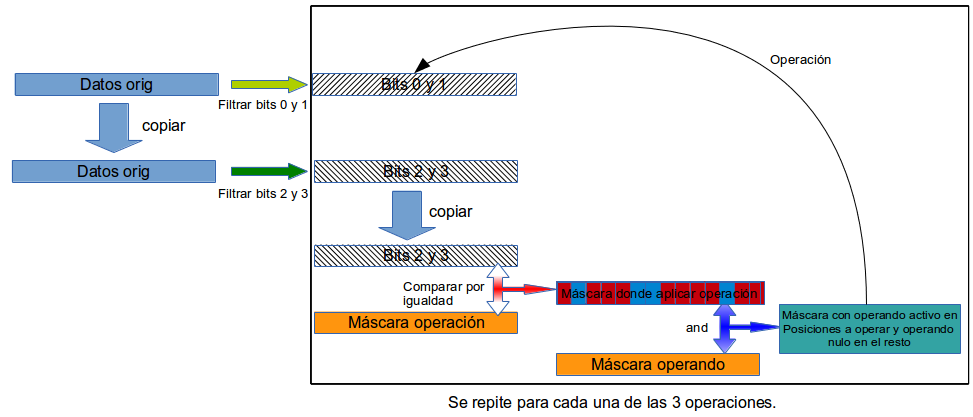
\includegraphics[scale=0.6]{secciones/decodificacion/imagenes/esquemaCicloDecode.png}
\end{center}
\caption{Esquema de funcionamiento de la primera parte del ciclo de decode.}
\label{fig:ciclo-decode}
\end{figure}


	Una vez hecho esto lo único que falta es acomodar los datos y grabarlos.

	Terminado todo esto se hacen avanzar los punteros y se mueven los datos que se
trajeron al registro xmm0 para poder procesarlos en la próxima iteración.

	A esta altura es importante remarcar una cosa que tal vez no se notó tanto.
El entubado de código en dos etapas (que aumentó el rendimiento en cerca del 15\%)
sólo agrega unas pocas líneas de código al ejercicio:


\begin{minted}[linenos,stepnumber=1]{nasm}

	MOVDQA xmm0, [rdi]

;(logica para la multiplicidad de size)

ciclo:

	MOVDQU xmm7, [rdi+r9] ; Se traen datos nuevos  se los guarda en un registro auxiliar

;---------------------------------------------------------------
;--------Cuerpo del ciclo usando los datos de xmm0--------------
;---------------------------------------------------------------

	MOVDQA xmm0, xmm7; Se dejan los datos en xmm0 para poder usarlos la proxima iteracion

;---------------------------------------------------------------
;--------Final del ciclo y logica para multiplicidad de size----
;---------------------------------------------------------------

\end{minted}

	Esas 3 líneas de código son las únicas realmente involucradas con
el entubado de código. Es decir que usar el entubado de código de esta forma
realmente tiene una gigantezca relación costo beneficio.



\newpage

\subsubsection{Implementación decode ASM: La multiplicidad de \textit{size}}

	El problema de la multiplicidad de size es un problema sencillo que
obliga a agregar mas lógica de la que pareciera. El problema en esta implementación
de este filtro es que se usan 2 contadores simultaneos (uno para \textit{src} y otro
para \textit{dst} ) y cada uno avanza a otra velocidad. Sin embargo \textit{size} se
compara con uno sólo de ellos para saber cuando parar de iterar, la consecuencia
de ello es que cuando la multiplicidad de size no es la adecuada hay que modificar
los dos contadores de manera diferente.

	La solución que se le dió a esta problemática en esta implementación está
dividida en 2 etapas: Antes de entrar al ciclo se calcula cuanto va a tener
que retroceder el contador de \textit{src}.

\begin{minted}[tabsize=4]{nasm}

	MOV    r8, rdx  ; Se copia size
	SHL    r8, 62   ; Se conservan los últimos 2 bits (resto módulo 4)		
	SHR    r8, 62   ; Se vuelve al estado original
	MOV    rcx, 4   ; En otro registro se trae un 4
	SUB    rcx, r8  ; Ahora en rcx está lo que falta a rdx para ser módulo 4
	SHL    rcx, 2   ; Finalmente se lo multiplica por 4. Esto es lo que queremos que
                    ; retroceda el contador de fuente que avanza 4 veces mas rápido
									
	ADD    rcx, 16  ; Se suma 16 a rcx para compensar que el contador siempre esta
                    ; una iteracion mas adelante que el proceso de datos por el
                    ; entubado de codigo

	XOR	   r8, r8 	; r8 se usa como flag al final del ciclo.						

\end{minted}


	La segunda parte es un sector del ciclo al que sólo se accede en la última
iteración. Basicamente lo que se hace es mover el límite de se hace es
poner al contador de \textit{dst} (r10) en la posición exacta a la que debe
quedar (\textit{size}-4) y hacer retroceder al contador de destino
con la cifra calculada antes. Además se cambia el flag indicando que ya
se pasó por ahí para que efectivamente sea la última iteración.



\begin{minted}[tabsize=4]{nasm}

	JL       ciclo           ; Final del ciclo

	MOV      r10, rdx        ; Se pone el contador de dst en size-4
	SUB      r9, rcx         ; Se hace retroceder el contador de src la cantidad adecuada
	MOVDQU   xmm0, [rdi+r9]  ; Se ponen en xmm0 los datos adecuados para la ultima iteracion
	CMP      r8, 0           ; Se verifica que sea la primera vez que se entra al ciclo.
	MOV      r8, 1           ; Se setea el flag en "ya se visito este lugar"
	JE       ciclo           ; Si el flag estaba en cero se salta a ciclo. 
                                ; (notar que MOV no modifica eflags)

\end{minted}


	Esta solución para este problema tiene como principal problema
que siempre se realiza una iteración de más, por mas que la multiplicidad
de \textit{size} sea la correcta. Sin embargo los ciclos
de este filtro son realmente muy rápidos, por lo que eso no resulta
un problema mayor.

\newpage

\subsection{Rendimiento}

\begin{figure}[h]
\begin{center}
  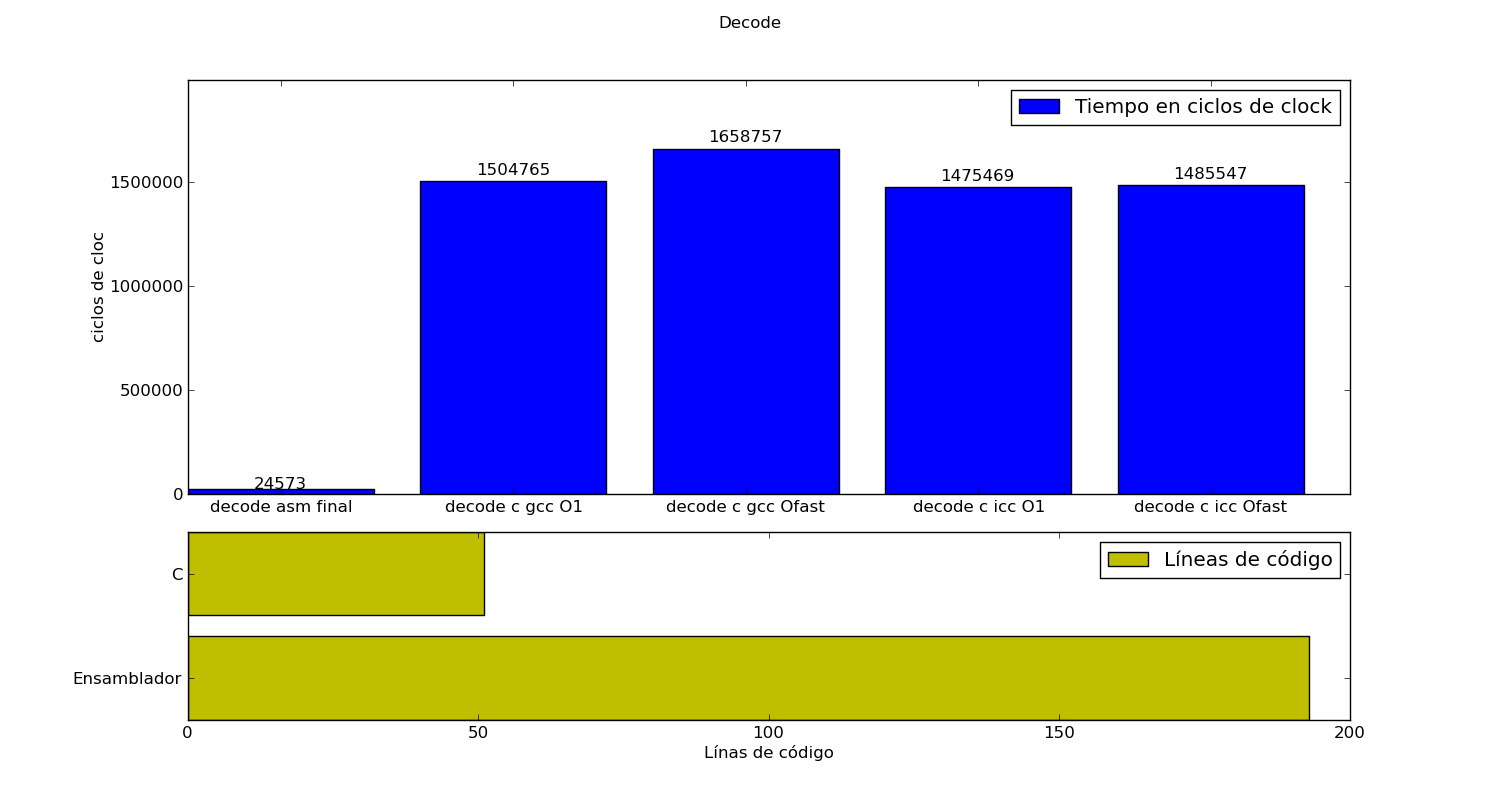
\includegraphics[scale=0.5]{secciones/decodificacion/imagenes/decode.png}
\end{center}
\caption{Imagen antes y después de aplicar el filtro de color con color principal rojo.}
\label{fig:rendimiento decode}
\end{figure}

	Como se puede ver en el gráfico el rendimiento de la versión en assembler es notablemente mas rápida. Otra
vez no cumple con la hipótesis inicial. La versión en ASM es más de 60 veces mas rápida que la versión
de C. Al introducir ICC en la ecuación la cosa cambia un poco, sin embargo el resultado sigue siendo que
la versión en ensamblador aplasta a las demás.

	En este momento cabe volver a mencionar que este filtro calza a la perfección en el procesamiento
SIMD con SSE. Aclarado esto vamos a ahondar un poco más.

	La versión de C siguiendo el código tal cuál está escrito accede a memoria 5 veces cada 4 bytes.
Es decir, tiene que buscar cada byte. Luego de procesar 4 bytes tiene que ir a guardarlos. Es decir
que suponiendo que el compilador genera un código que no accede nunca a memoria durante el ciclo de todas
maneras se están accediendo 20 veces a memoria cada 16 bytes. La versión escita en ensamblador, en cambio
realiza sólo 2 accesos cada 16 bytes (uno para traer datos, otro para guardarlos). Pero no sólo eso sino
que además el acceso mas conflictivo (el de trar datos) está optimizado mediante entubado de código.

	Otra cosa importante a la hora de hacer este análisis es que se sabe con mucha presición
cuantas veces se realiza el ciclo principal. Si o si está en el orden de $size/4$ veces. Es decir,
en cada iteración se graban exactamente 4 bytes y las iteraciones terminan cuando se graban $size$
por lo tanto ese va a ser el total de iteraciones.

	Despreciando las instrucciones de afuera del ciclo (que tiene sentido porque son pocas y se
realizan una sóla vez) la cantidad de ciclos de clock por iteración entonces va a ser el cociente
entre los clocks totales y $size/4$. Eso da proximamente 9,2. Sin embargo el ciclo tiene 36
instrucciones, lo que quiere decir que se logró aproximadamente un rendimiento de 4 instrucciones
por ciclo de clock.


	\newpage

	\section{Conclusiones}
		\begin{comment}
	- ¿Valió la pena?
		- Evaluar costo de implementación vs performance.
		- Evaluar si el aumento de performance tiene o no sentido. (Caso decode, es bien al pedo. Sin embargo en aplicaciones de tiempo real o de uso masivo tiene mucho sentido porque el aumento es muy significativo).
		- 
	- ¿Cuánto pesa el uso óptimo del hardware vs el algorítmo?
		- Explicar por qué el algoritmo de fondo es el mismo concluyendo que un mejor uso del hardware puede lograr incrementos sumamente significativos.
	- ¿Se llegó a cambiar el orden de magnitud?
		- Si bien obviamente no se llegó orden de complejidad si aumenta el orden de magnitud en cuanto a velocidad de ejecución. Decode y miniature.

\end{comment}


	
\end{document}
